% QuizForge Complete Backend Documentation
% Main Document
\documentclass[12pt,a4paper]{report}

% Packages
\usepackage[utf8]{inputenc}
\usepackage[T1]{fontenc}
\usepackage{geometry}
\usepackage{graphicx}
\usepackage{tikz}
\usetikzlibrary{shapes.multipart, positioning, arrows.meta, calc}
\usepackage{listings}
\usepackage{xcolor}
\usepackage{hyperref}
\usepackage{tcolorbox}
\usepackage{fancyhdr}
\usepackage{titlesec}
\usepackage{longtable}
\usepackage{array}
\usepackage{booktabs}
\usepackage{enumitem}
\usepackage{pdflscape}

% Page geometry
\geometry{
    a4paper,
    left=25mm,
    right=25mm,
    top=30mm,
    bottom=30mm
}

% Colors
\definecolor{codegreen}{rgb}{0,0.6,0}
\definecolor{codegray}{rgb}{0.5,0.5,0.5}
\definecolor{codepurple}{rgb}{0.58,0,0.82}
\definecolor{backcolour}{rgb}{0.95,0.95,0.92}
\definecolor{javakey}{rgb}{0.5,0,0.35}

% Code listing style
\lstdefinestyle{javastyle}{
    backgroundcolor=\color{backcolour},
    commentstyle=\color{codegreen},
    keywordstyle=\color{javakey}\bfseries,
    numberstyle=\tiny\color{codegray},
    stringstyle=\color{codepurple},
    basicstyle=\ttfamily\footnotesize,
    breakatwhitespace=false,
    breaklines=true,
    captionpos=b,
    keepspaces=true,
    numbers=left,
    numbersep=5pt,
    showspaces=false,
    showstringspaces=false,
    showtabs=false,
    tabsize=2,
    frame=single,
    language=Java
}

\lstset{style=javastyle}

% Hyperref setup
\hypersetup{
    colorlinks=true,
    linkcolor=blue,
    filecolor=magenta,
    urlcolor=cyan,
    pdftitle={QuizForge Backend Documentation},
    pdfauthor={System Documentation},
    pdfsubject={Complete Backend Analysis},
}

% Headers and footers
\pagestyle{fancy}
\fancyhf{}
\fancyhead[L]{\leftmark}
\fancyhead[R]{QuizForge Backend}
\fancyfoot[C]{\thepage}

% Title formatting
\titleformat{\chapter}[display]
{\normalfont\huge\bfseries}{\chaptertitlename\ \thechapter}{20pt}{\Huge}

% Document metadata
\title{%
    \Huge\textbf{QuizForge} \\
    \Large Complete Backend Documentation \\
    \large Version 1.0.0
}
\author{Technical Documentation}
\date{\today}

\begin{document}

% Title page
\maketitle
\tableofcontents
\newpage

% Include all sections
% Chapter 1: Introduction
\chapter{Introduction}

\section{Project Overview}

\textbf{QuizForge} is an online quiz platform built with a modern technology stack, providing a comprehensive solution for quiz creation, management, and assessment. The platform supports role-based access control with two distinct user types: Administrators and Candidates.

\subsection{Key Features}

\begin{itemize}[leftmargin=*]
    \item \textbf{Role-Based Access Control (RBAC):} Separate functionalities for ADMIN and CANDIDATE roles
    \item \textbf{Quiz Management:} Create, read, update, and delete quizzes with multiple question types
    \item \textbf{Real-Time Quiz Taking:} Candidates can take quizzes with time tracking
    \item \textbf{Automatic Grading:} System automatically evaluates multiple-choice and true/false questions
    \item \textbf{Analytics Dashboard:} Comprehensive statistics for quiz performance
    \item \textbf{RESTful API:} Complete REST API with OpenAPI 3.0 documentation
    \item \textbf{JWT Authentication:} Secure token-based authentication system
\end{itemize}

\section{Technology Stack}

\subsection{Backend Technologies}

\begin{table}[h]
\centering
\begin{tabular}{|l|l|p{6cm}|}
\hline
\textbf{Technology} & \textbf{Version} & \textbf{Purpose} \\
\hline
Java & 21 & Core programming language \\
\hline
Spring Boot & 3.2.0 & Application framework \\
\hline
Spring Security & 3.2.0 & Authentication and authorization \\
\hline
Spring Data JPA & 3.2.0 & Data persistence layer \\
\hline
PostgreSQL & Latest & Relational database \\
\hline
JWT (JJWT) & 0.11.5 & Token-based authentication \\
\hline
SpringDoc OpenAPI & 2.6.0 & API documentation \\
\hline
Lombok & Latest & Reduce boilerplate code \\
\hline
Bean Validation & 3.2.0 & Input validation \\
\hline
\end{tabular}
\caption{Backend Technology Stack}
\end{table}

\section{Project Structure}

The project follows a standard Spring Boot layered architecture:

\begin{verbatim}
quizforge/
|------ backend/
|   |------ pom.xml                      # Maven configuration
|   \`------ src/main/java/com/quizforge/
|       |------ QuizForgeApplication.java
|       |------ config/                  # Configuration classes
|       |   \`------ OpenApiConfig.java
|       |------ controller/              # REST endpoints
|       |   |------ AuthController.java
|       |   |------ AdminController.java
|       |   \`------ CandidateController.java
|       |------ dto/                     # Data Transfer Objects
|       |------ model/                   # JPA Entities
|       |------ repository/              # Data access layer
|       |------ security/                # Security configuration
|       \`------ service/                 # Business logic
\`------ frontend/                        # React frontend
\end{verbatim}

\section{Design Patterns}

The application implements several industry-standard design patterns:

\begin{enumerate}
    \item \textbf{MVC (Model-View-Controller):} Separation of concerns between data, business logic, and presentation
    \item \textbf{Repository Pattern:} Abstraction layer for data access operations
    \item \textbf{Service Layer Pattern:} Business logic encapsulation
    \item \textbf{DTO Pattern:} Data transfer between layers
    \item \textbf{Builder Pattern:} Used by Lombok for object construction
    \item \textbf{Filter Chain Pattern:} JWT authentication filter
    \item \textbf{Singleton Pattern:} Spring beans are singletons by default
\end{enumerate}

\section{API Architecture}

The API follows RESTful principles with the following characteristics:

\begin{itemize}
    \item \textbf{Resource-Based URLs:} Endpoints represent resources (users, quizzes, attempts)
    \item \textbf{HTTP Methods:} Proper use of GET, POST, PUT, DELETE
    \item \textbf{Stateless:} Each request contains all necessary information
    \item \textbf{JSON Format:} All data exchanged in JSON format
    \item \textbf{HTTP Status Codes:} Meaningful status codes (200, 201, 400, 401, 404, etc.)
    \item \textbf{HATEOAS-Ready:} Structure supports hypermedia links
\end{itemize}

\section{Database Schema Overview}

The application uses six main entities:

\begin{enumerate}
    \item \textbf{User:} Stores user information with role-based access
    \item \textbf{Quiz:} Main quiz entity with metadata
    \item \textbf{Question:} Individual questions belonging to quizzes
    \item \textbf{Option:} Multiple choice options for questions
    \item \textbf{QuizAttempt:} Tracks user quiz attempts
    \item \textbf{Answer:} Stores user responses to questions
\end{enumerate}

\section{Document Organization}

This documentation is organized into the following chapters:

\begin{description}
    \item[Chapter 2: Architecture] Overall system architecture and design decisions
    \item[Chapter 3: Models] Detailed explanation of JPA entities
    \item[Chapter 4: Repositories] Data access layer analysis
    \item[Chapter 5: Services] Business logic implementation
    \item[Chapter 6: Controllers] REST API endpoints
    \item[Chapter 7: Security] Authentication and authorization
    \item[Chapter 8: API Documentation] Complete OpenAPI specification
    \item[Chapter 9: ER Diagram] Database relationships and design
    \item[Chapter 10: Configuration] Application configuration details
    \item[Appendix A: Dependencies] Complete dependency list and versions
\end{description}

\section{Conventions Used in This Document}

\begin{tcolorbox}[title=Code Conventions]
\begin{itemize}
    \item \texttt{Monospace font} indicates code, class names, or file paths
    \item \textbf{Bold text} highlights important concepts
    \item \textit{Italic text} indicates technical terms
    \item Code listings include line numbers for reference
\end{itemize}
\end{tcolorbox}


% Chapter 2: Architecture
\chapter{System Architecture}

\section{Layered Architecture}

QuizForge implements a classic n-tier architecture with clear separation of concerns:

\begin{figure}[h]
\centering
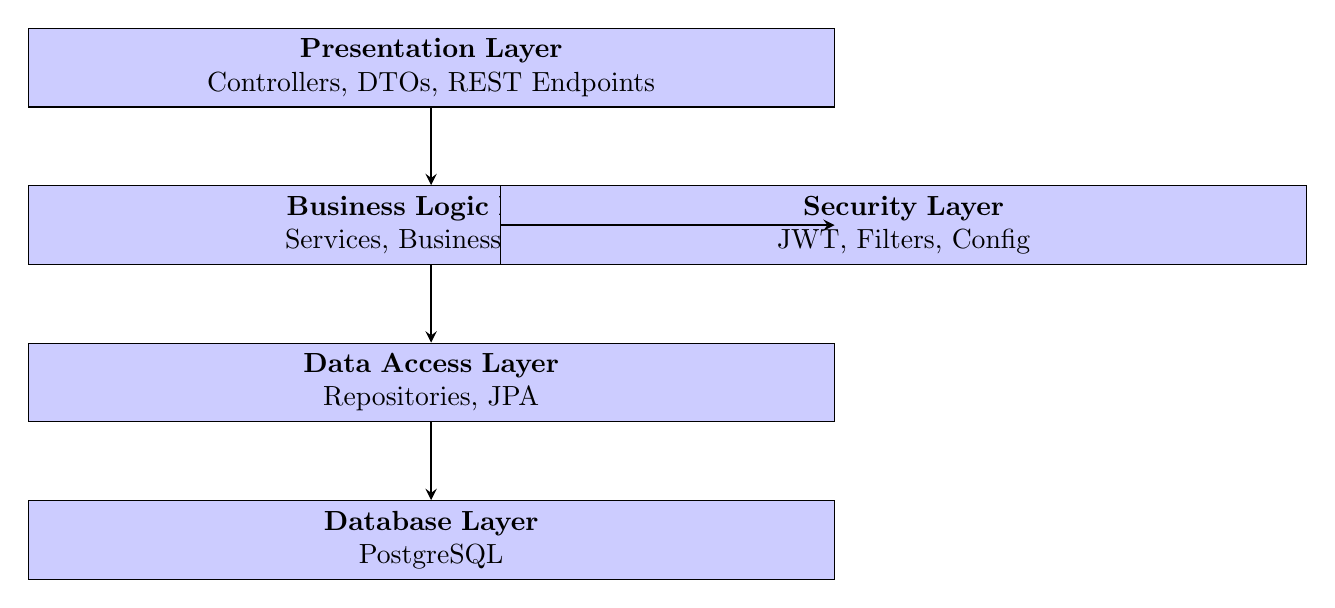
\begin{tikzpicture}[
    layer/.style={rectangle, draw, fill=blue!20, text width=10cm, text centered, minimum height=1cm},
    arrow/.style={->, >=stealth, thick}
]
    \node[layer] (presentation) at (0,0) {\textbf{Presentation Layer} \\ Controllers, DTOs, REST Endpoints};
    \node[layer] (business) at (0,-2) {\textbf{Business Logic Layer} \\ Services, Business Rules};
    \node[layer] (data) at (0,-4) {\textbf{Data Access Layer} \\ Repositories, JPA};
    \node[layer] (database) at (0,-6) {\textbf{Database Layer} \\ PostgreSQL};
    \node[layer] (security) at (6,-2) {\textbf{Security Layer} \\ JWT, Filters, Config};
    
    \draw[arrow] (presentation) -- (business);
    \draw[arrow] (business) -- (data);
    \draw[arrow] (data) -- (database);
    \draw[arrow] (security) -- (business);
\end{tikzpicture}
\caption{System Architecture Layers}
\end{figure}

\subsection{Layer Responsibilities}

\subsubsection{Presentation Layer}
\begin{itemize}
    \item \textbf{Controllers:} Handle HTTP requests and responses
    \item \textbf{DTOs:} Transfer data between client and server
    \item \textbf{Validation:} Input validation using Bean Validation
    \item \textbf{Error Handling:} Exception handling and error responses
\end{itemize}

\subsubsection{Business Logic Layer}
\begin{itemize}
    \item \textbf{Services:} Implement core business logic
    \item \textbf{Transactions:} Manage database transactions
    \item \textbf{Data Transformation:} Convert between entities and DTOs
    \item \textbf{Business Rules:} Enforce application rules and constraints
\end{itemize}

\subsubsection{Data Access Layer}
\begin{itemize}
    \item \textbf{Repositories:} Abstract database operations
    \item \textbf{JPA Entities:} Map to database tables
    \item \textbf{Query Methods:} Define custom queries
    \item \textbf{Relationship Management:} Handle entity associations
\end{itemize}

\subsubsection{Security Layer}
\begin{itemize}
    \item \textbf{JWT Authentication:} Token generation and validation
    \item \textbf{Authorization:} Role-based access control
    \item \textbf{Filters:} Request/response interception
    \item \textbf{CORS:} Cross-origin resource sharing
\end{itemize}

\section{Request Flow}

The typical request flow through the application:

\begin{enumerate}
    \item \textbf{Client Request:} HTTP request arrives at the server
    \item \textbf{JWT Filter:} JwtRequestFilter validates the JWT token
    \item \textbf{Security Context:} Authentication is set in SecurityContext
    \item \textbf{Controller:} Request is routed to appropriate controller method
    \item \textbf{Validation:} Input is validated against constraints
    \item \textbf{Service Layer:} Business logic is executed
    \item \textbf{Repository:} Database operations are performed
    \item \textbf{Response:} DTO is created and returned to client
\end{enumerate}

\begin{figure}[h]
\centering
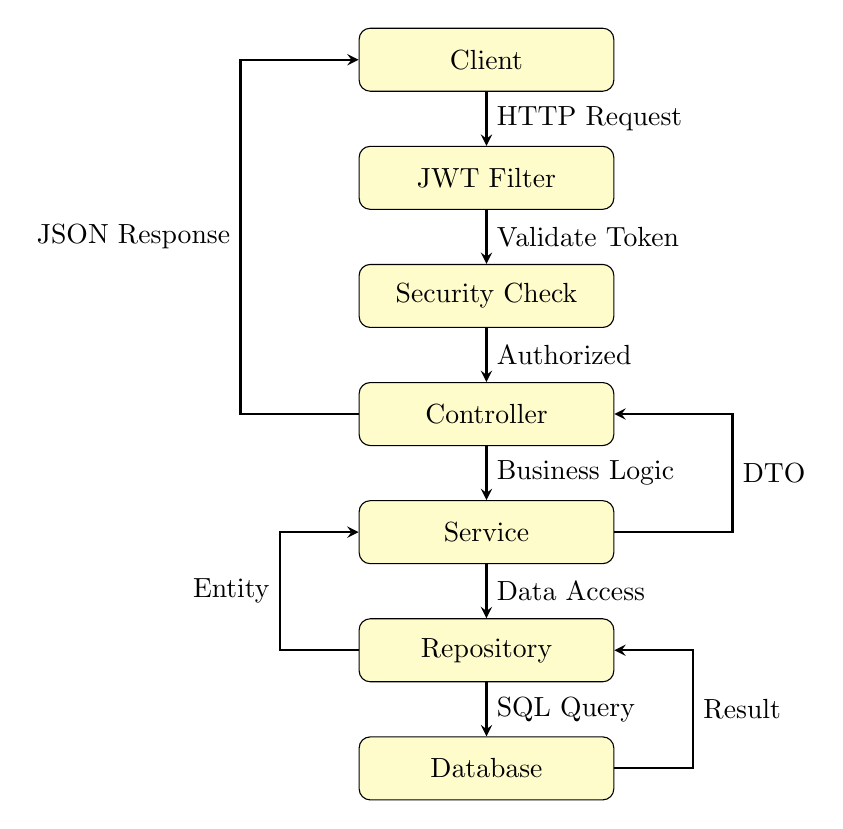
\begin{tikzpicture}[
    node distance=1.5cm,
    box/.style={rectangle, draw, fill=yellow!20, text width=3cm, text centered, minimum height=0.8cm, rounded corners},
    arrow/.style={->, >=stealth, thick}
]
    \node[box] (client) {Client};
    \node[box, below of=client] (filter) {JWT Filter};
    \node[box, below of=filter] (security) {Security Check};
    \node[box, below of=security] (controller) {Controller};
    \node[box, below of=controller] (service) {Service};
    \node[box, below of=service] (repository) {Repository};
    \node[box, below of=repository] (database) {Database};
    
    \draw[arrow] (client) -- node[right] {HTTP Request} (filter);
    \draw[arrow] (filter) -- node[right] {Validate Token} (security);
    \draw[arrow] (security) -- node[right] {Authorized} (controller);
    \draw[arrow] (controller) -- node[right] {Business Logic} (service);
    \draw[arrow] (service) -- node[right] {Data Access} (repository);
    \draw[arrow] (repository) -- node[right] {SQL Query} (database);
    
    \draw[arrow] (database.east) -- ++(1,0) |- node[right, near start] {Result} (repository.east);
    \draw[arrow] (repository.west) -- ++(-1,0) |- node[left, near start] {Entity} (service.west);
    \draw[arrow] (service.east) -- ++(1.5,0) |- node[right, near start] {DTO} (controller.east);
    \draw[arrow] (controller.west) -- ++(-1.5,0) |- node[left, near start] {JSON Response} (client.west);
\end{tikzpicture}
\caption{Request Flow Diagram}
\end{figure}

\section{Component Interaction}

\subsection{Authentication Flow}

\begin{lstlisting}[caption=Authentication Sequence]
1. User sends credentials to /api/auth/login
2. AuthController receives request
3. AuthService validates credentials (simplified for demo)
4. JwtUtil generates JWT token with role
5. LoginResponse with token returned to user
6. User includes token in Authorization header for subsequent requests
7. JwtRequestFilter extracts and validates token
8. SecurityContext populated with authentication
9. Request proceeds to controller with authenticated user
\end{lstlisting}

\subsection{Quiz Creation Flow}

\begin{lstlisting}[caption=Quiz Creation Sequence]
1. Admin sends POST request to /api/admin/quizzes
2. JWT filter validates admin role
3. AdminController receives QuizRequest
4. Bean validation checks input constraints
5. AdminService.createQuiz() called
6. User entity fetched or created
7. Quiz entity created with questions and options
8. CascadeType.ALL persists entire object graph
9. QuizRepository.save() persists to database
10. Entity converted to QuizResponse DTO
11. JSON response returned to client
\end{lstlisting}

\subsection{Quiz Taking Flow}

\begin{lstlisting}[caption=Quiz Taking Sequence]
1. Candidate requests quiz list: GET /api/candidate/quizzes
2. Active quizzes returned without correct answers
3. Candidate starts quiz: POST /api/candidate/quizzes/{id}/start
4. QuizAttempt entity created with IN_PROGRESS status
5. Candidate retrieves questions: GET /api/candidate/quizzes/{id}
6. Questions returned with options (isCorrect hidden)
7. Candidate submits answers: POST /api/candidate/quizzes/submit
8. Answers evaluated against correct options
9. Score calculated and QuizAttempt updated to EVALUATED
10. Results returned to candidate
\end{lstlisting}

\section{Design Decisions}

\subsection{Why Spring Boot 3.2.0?}

\begin{itemize}
    \item Native support for Java 21 features
    \item Enhanced observability and monitoring
    \item Improved startup time and memory efficiency
    \item Built-in support for modern standards
    \item Jakarta EE 10 migration complete
\end{itemize}

\subsection{Why PostgreSQL?}

\begin{itemize}
    \item ACID compliance for data integrity
    \item Advanced indexing capabilities
    \item JSON support for flexible data
    \item Excellent performance with JPA
    \item Wide community support
\end{itemize}

\subsection{Why JWT Authentication?}

\begin{itemize}
    \item Stateless authentication (no server-side sessions)
    \item Scalable across multiple servers
    \item Works well with SPAs and mobile apps
    \item Industry-standard approach
    \item Easy to implement role-based access
\end{itemize}

\subsection{Why Lombok?}

\begin{itemize}
    \item Reduces boilerplate code significantly
    \item Automatic getters, setters, constructors
    \item Builder pattern implementation
    \item Cleaner, more readable code
    \item Compile-time code generation
\end{itemize}

\section{Scalability Considerations}

\subsection{Horizontal Scalability}
\begin{itemize}
    \item Stateless JWT authentication enables load balancing
    \item No session affinity required
    \item Database connection pooling
    \item Can deploy multiple instances behind load balancer
\end{itemize}

\subsection{Database Optimization}
\begin{itemize}
    \item Lazy loading for relationships (LAZY fetch type)
    \item Indexed columns for frequent queries
    \item Batch operations for bulk inserts
    \item Connection pool configuration
\end{itemize}

\subsection{Caching Opportunities}
\begin{itemize}
    \item Quiz data (rarely changes)
    \item User information
    \item Query results for analytics
    \item Second-level cache with Hibernate
\end{itemize}

\section{Error Handling Strategy}

The application handles errors at multiple levels:

\begin{enumerate}
    \item \textbf{Validation Errors:} Bean Validation catches invalid inputs
    \item \textbf{Business Logic Errors:} Services throw RuntimeException with messages
    \item \textbf{Security Errors:} JWT filter returns 401 Unauthorized
    \item \textbf{Database Errors:} JPA handles constraint violations
    \item \textbf{Global Exception Handler:} Can be added for centralized error handling
\end{enumerate}

\section{Transaction Management}

Spring's declarative transaction management is used:

\begin{itemize}
    \item \texttt{@Transactional} annotation on service methods
    \item Automatic rollback on RuntimeException
    \item Propagation defaults to REQUIRED
    \item Isolation level defaults to database default
\end{itemize}


% Chapter 3: Models (Part 1)
\chapter{Data Models (JPA Entities)}

\section{Overview}

The application uses six JPA entities that map to PostgreSQL database tables. These entities form the core data model and define the relationships between different domain objects.

\section{User Entity}

\subsection{Purpose}
The \texttt{User} entity represents system users with role-based access control. It supports two roles: ADMIN and CANDIDATE.

\subsection{Complete Source Code}

\begin{lstlisting}[caption=User.java - Complete Implementation]
package com.quizforge.model;

import jakarta.persistence.*;
import lombok.AllArgsConstructor;
import lombok.Data;
import lombok.NoArgsConstructor;

import java.time.LocalDateTime;

@Entity
@Table(name = ''users'')
@Data
@NoArgsConstructor
@AllArgsConstructor
public class User {
    @Id
    @GeneratedValue(strategy = GenerationType.IDENTITY)
    private Long id;

    @Column(nullable = false, unique = true)
    private String email;

    @Column(nullable = false)
    private String password;

    @Column(nullable = false)
    private String name;

    @Enumerated(EnumType.STRING)
    @Column(nullable = false)
    private Role role;

    @Column(name = ''created_at'', nullable = false, updatable = false)
    private LocalDateTime createdAt;

    @PrePersist
    protected void onCreate() {
        createdAt = LocalDateTime.now();
    }

    public enum Role {
        ADMIN, CANDIDATE
    }
}
\end{lstlisting}

\subsection{Line-by-Line Explanation}

\begin{itemize}[leftmargin=*]
    \item \textbf{Line 1-7:} Package declaration and imports
    \begin{itemize}
        \item \texttt{jakarta.persistence.*}: JPA annotations for entity mapping
        \item \texttt{lombok.*}: Code generation annotations
        \item \texttt{java.time.LocalDateTime}: For timestamp fields
    \end{itemize}
    
    \item \textbf{Line 9: @Entity}
    \begin{itemize}
        \item Marks this class as a JPA entity
        \item Will be managed by EntityManager
        \item Participates in persistence lifecycle
    \end{itemize}
    
    \item \textbf{Line 10: @Table(name = ''users'')}
    \begin{itemize}
        \item Maps entity to ''users'' table in database
        \item If omitted, table name would default to ''User''
        \item ''users'' avoids potential reserved word conflicts
    \end{itemize}
    
    \item \textbf{Line 11: @Data}
    \begin{itemize}
        \item Lombok annotation generating: getters, setters, toString(), equals(), hashCode()
        \item Reduces boilerplate code significantly
        \item Generated at compile time
    \end{itemize}
    
    \item \textbf{Line 12-13: @NoArgsConstructor, @AllArgsConstructor}
    \begin{itemize}
        \item Generate no-args and all-args constructors
        \item Required by JPA for entity instantiation
        \item Useful for creating instances in application code
    \end{itemize}
    
    \item \textbf{Line 15-17: Primary Key}
    \begin{itemize}
        \item \texttt{@Id}: Marks field as primary key
        \item \texttt{@GeneratedValue(strategy = GenerationType.IDENTITY)}: Auto-increment by database
        \item \texttt{Long id}: Surrogate key, nullable until persisted
    \end{itemize}
    
    \item \textbf{Line 19-20: Email Field}
    \begin{itemize}
        \item \texttt{nullable = false}: NOT NULL constraint in database
        \item \texttt{unique = true}: UNIQUE constraint, enforces no duplicates
        \item Used as username for authentication
    \end{itemize}
    
    \item \textbf{Line 22-23: Password Field}
    \begin{itemize}
        \item Stores user password
        \item Should be encrypted (BCrypt) in production
        \item Currently simplified for demo purposes
    \end{itemize}
    
    \item \textbf{Line 25-26: Name Field}
    \begin{itemize}
        \item Display name for the user
        \item Required field (nullable = false)
    \end{itemize}
    
    \item \textbf{Line 28-30: Role Field (Enum)}
    \begin{itemize}
        \item \texttt{@Enumerated(EnumType.STRING)}: Store enum name as string in DB
        \item Alternative is \texttt{EnumType.ORDINAL} (stores integer)
        \item STRING is preferred for maintainability
        \item Controls access to different API endpoints
    \end{itemize}
    
    \item \textbf{Line 32-33: Created At Timestamp}
    \begin{itemize}
        \item \texttt{name = ''created\_at''}: Column name in database (snake\_case)
        \item \texttt{updatable = false}: Prevents changes after initial insert
        \item Records when user was created
    \end{itemize}
    
    \item \textbf{Line 35-38: @PrePersist Callback}
    \begin{itemize}
        \item JPA lifecycle callback executed before INSERT
        \item Automatically sets createdAt to current timestamp
        \item Ensures consistent timestamp generation
        \item Called by EntityManager during persist operation
    \end{itemize}
    
    \item \textbf{Line 40-42: Role Enum}
    \begin{itemize}
        \item Defines two possible roles: ADMIN, CANDIDATE
        \item ADMIN: Can create, edit, delete quizzes; view analytics
        \item CANDIDATE: Can take quizzes and view results
        \item Used by Spring Security for authorization
    \end{itemize}
\end{itemize}

\subsection{Database Table Structure}

\begin{table}[h]
\centering
\begin{tabular}{|l|l|l|l|}
\hline
\textbf{Column} & \textbf{Type} & \textbf{Constraints} & \textbf{Description} \\
\hline
id & BIGSERIAL & PRIMARY KEY & Auto-increment ID \\
email & VARCHAR(255) & NOT NULL, UNIQUE & User email/username \\
password & VARCHAR(255) & NOT NULL & Encrypted password \\
name & VARCHAR(255) & NOT NULL & Display name \\
role & VARCHAR(50) & NOT NULL & ADMIN or CANDIDATE \\
created\_at & TIMESTAMP & NOT NULL & Creation timestamp \\
\hline
\end{tabular}
\caption{Users Table Structure}
\end{table}

\subsection{Relationships}
\begin{itemize}
    \item One User to Many Quizzes (as creator)
    \item One User to Many QuizAttempts (as candidate)
\end{itemize}

\section{Quiz Entity}

\subsection{Purpose}
The \texttt{Quiz} entity represents a quiz with metadata and associated questions. Admins create quizzes that candidates can take.

\subsection{Complete Source Code}

\begin{lstlisting}[caption=Quiz.java - Complete Implementation]
package com.quizforge.model;

import jakarta.persistence.*;
import lombok.AllArgsConstructor;
import lombok.Data;
import lombok.NoArgsConstructor;

import java.time.LocalDateTime;
import java.util.ArrayList;
import java.util.List;

@Entity
@Table(name = ''quizzes'')
@Data
@NoArgsConstructor
@AllArgsConstructor
public class Quiz {
    @Id
    @GeneratedValue(strategy = GenerationType.IDENTITY)
    private Long id;

    @Column(nullable = false)
    private String title;

    @Column(columnDefinition = ''TEXT'')
    private String description;

    @Column(nullable = false)
    private Integer duration; // in minutes

    @Column(nullable = false)
    private Boolean isActive = true;

    @ManyToOne(fetch = FetchType.LAZY)
    @JoinColumn(name = ''created_by'', nullable = false)
    private User createdBy;

    @OneToMany(mappedBy = ''quiz'', cascade = CascadeType.ALL, 
               orphanRemoval = true)
    private List<Question> questions = new ArrayList<>();

    @Column(name = ''created_at'', nullable = false, updatable = false)
    private LocalDateTime createdAt;

    @Column(name = ''updated_at'')
    private LocalDateTime updatedAt;

    @PrePersist
    protected void onCreate() {
        createdAt = LocalDateTime.now();
        updatedAt = LocalDateTime.now();
    }

    @PreUpdate
    protected void onUpdate() {
        updatedAt = LocalDateTime.now();
    }
}
\end{lstlisting}

\subsection{Line-by-Line Explanation}

\begin{itemize}[leftmargin=*]
    \item \textbf{Line 18-20: Primary Key}
    \begin{itemize}
        \item Auto-generated ID using IDENTITY strategy
        \item Unique identifier for each quiz
    \end{itemize}
    
    \item \textbf{Line 22-23: Title Field}
    \begin{itemize}
        \item Quiz name/title
        \item Required field (nullable = false)
        \item Displayed to users in quiz listings
    \end{itemize}
    
    \item \textbf{Line 25-26: Description Field}
    \begin{itemize}
        \item \texttt{columnDefinition = ''TEXT''}: Uses TEXT type instead of VARCHAR
        \item Allows longer descriptions without length limits
        \item Optional field (can be null)
        \item Provides context about quiz content
    \end{itemize}
    
    \item \textbf{Line 28-29: Duration Field}
    \begin{itemize}
        \item Time limit for quiz in minutes
        \item Integer type for simplicity
        \item Required field
        \item Used to calculate quiz deadline
    \end{itemize}
    
    \item \textbf{Line 31-32: IsActive Field}
    \begin{itemize}
        \item Boolean flag to enable/disable quiz
        \item Defaults to true
        \item Only active quizzes shown to candidates
        \item Allows soft deactivation without deletion
    \end{itemize}
    
    \item \textbf{Line 34-36: CreatedBy Relationship}
    \begin{itemize}
        \item \texttt{@ManyToOne}: Many quizzes can be created by one user
        \item \texttt{fetch = FetchType.LAZY}: User loaded only when accessed
        \item \texttt{@JoinColumn(name = ''created\_by'')}: Foreign key column name
        \item \texttt{nullable = false}: Every quiz must have a creator
        \item References User entity
    \end{itemize}
    
    \item \textbf{Line 38-40: Questions Relationship}
    \begin{itemize}
        \item \texttt{@OneToMany}: One quiz has many questions
        \item \texttt{mappedBy = ''quiz''}: Bidirectional relationship, Question owns FK
        \item \texttt{cascade = CascadeType.ALL}: All operations cascade to questions
        \item \texttt{orphanRemoval = true}: Delete questions if removed from list
        \item \texttt{new ArrayList<>()}: Initialize to avoid NullPointerException
    \end{itemize}
    
    \item \textbf{Line 42-43: CreatedAt Timestamp}
    \begin{itemize}
        \item Records when quiz was created
        \item Immutable (updatable = false)
    \end{itemize}
    
    \item \textbf{Line 45-46: UpdatedAt Timestamp}
    \begin{itemize}
        \item Tracks last modification time
        \item Can be updated on every change
    \end{itemize}
    
    \item \textbf{Line 48-52: @PrePersist Callback}
    \begin{itemize}
        \item Executed before INSERT operation
        \item Sets both createdAt and updatedAt
        \item Ensures timestamps are always set
    \end{itemize}
    
    \item \textbf{Line 54-57: @PreUpdate Callback}
    \begin{itemize}
        \item Executed before UPDATE operation
        \item Updates only updatedAt timestamp
        \item createdAt remains unchanged
    \end{itemize}
\end{itemize}

\subsection{Database Table Structure}

\begin{table}[h]
\centering
\begin{tabular}{|l|l|l|l|}
\hline
\textbf{Column} & \textbf{Type} & \textbf{Constraints} & \textbf{Description} \\
\hline
id & BIGSERIAL & PRIMARY KEY & Auto-increment ID \\
title & VARCHAR(255) & NOT NULL & Quiz title \\
description & TEXT & NULL & Quiz description \\
duration & INTEGER & NOT NULL & Time limit (minutes) \\
is\_active & BOOLEAN & NOT NULL & Active status \\
created\_by & BIGINT & NOT NULL, FK & Creator user ID \\
created\_at & TIMESTAMP & NOT NULL & Creation time \\
updated\_at & TIMESTAMP & NULL & Last update time \\
\hline
\end{tabular}
\caption{Quizzes Table Structure}
\end{table}

\subsection{Cascade Operations}

The \texttt{CascadeType.ALL} on questions means:
\begin{itemize}
    \item \textbf{PERSIST:} Saving quiz saves all questions
    \item \textbf{MERGE:} Updating quiz updates all questions
    \item \textbf{REMOVE:} Deleting quiz deletes all questions
    \item \textbf{REFRESH:} Refreshing quiz refreshes all questions
    \item \textbf{DETACH:} Detaching quiz detaches all questions
\end{itemize}


% Chapter 3 Continued: Models (Part 2)

\section{Question Entity}

\subsection{Purpose}
The \texttt{Question} entity represents individual questions within a quiz. Supports multiple question types including multiple-choice, true/false, and short answer.

\subsection{Complete Source Code}

\begin{lstlisting}[caption=Question.java - Complete Implementation]
package com.quizforge.model;

import jakarta.persistence.*;
import lombok.AllArgsConstructor;
import lombok.Data;
import lombok.NoArgsConstructor;

import java.util.ArrayList;
import java.util.List;

@Entity
@Table(name = ''questions'')
@Data
@NoArgsConstructor
@AllArgsConstructor
public class Question {
    @Id
    @GeneratedValue(strategy = GenerationType.IDENTITY)
    private Long id;

    @ManyToOne(fetch = FetchType.LAZY)
    @JoinColumn(name = ''quiz_id'', nullable = false)
    private Quiz quiz;

    @Column(nullable = false, columnDefinition = ''TEXT'')
    private String questionText;

    @Enumerated(EnumType.STRING)
    @Column(nullable = false)
    private QuestionType type;

    @Column(nullable = false)
    private Integer points = 1;

    @OneToMany(mappedBy = ''question'', cascade = CascadeType.ALL, 
               orphanRemoval = true)
    private List<Option> options = new ArrayList<>();

    public enum QuestionType {
        MULTIPLE_CHOICE, TRUE_FALSE, SHORT_ANSWER
    }
}
\end{lstlisting}

\subsection{Line-by-Line Explanation}

\begin{itemize}[leftmargin=*]
    \item \textbf{Line 21-23: Quiz Relationship}
    \begin{itemize}
        \item \texttt{@ManyToOne}: Many questions belong to one quiz
        \item \texttt{LAZY} fetch: Quiz loaded only when accessed
        \item \texttt{quiz\_id}: Foreign key column in database
        \item Question cannot exist without a quiz (nullable = false)
    \end{itemize}
    
    \item \textbf{Line 25-26: QuestionText Field}
    \begin{itemize}
        \item Stores the actual question text
        \item TEXT type for long questions
        \item Required field
    \end{itemize}
    
    \item \textbf{Line 28-30: Type Field (Enum)}
    \begin{itemize}
        \item \texttt{MULTIPLE\_CHOICE}: Question with multiple options, one correct
        \item \texttt{TRUE\_FALSE}: Binary question with two options
        \item \texttt{SHORT\_ANSWER}: Text-based answer (manual grading)
        \item Stored as string in database for readability
    \end{itemize}
    
    \item \textbf{Line 32-33: Points Field}
    \begin{itemize}
        \item Score value for this question
        \item Defaults to 1 point
        \item Used in calculating total quiz score
        \item Can be customized per question
    \end{itemize}
    
    \item \textbf{Line 35-37: Options Relationship}
    \begin{itemize}
        \item \texttt{@OneToMany}: One question has many options
        \item \texttt{mappedBy = ''question''}: Bidirectional relationship
        \item \texttt{CascadeType.ALL}: All operations cascade to options
        \item \texttt{orphanRemoval}: Delete options if removed from list
        \item Multiple choice questions typically have 4-5 options
    \end{itemize}
    
    \item \textbf{Line 39-41: QuestionType Enum}
    \begin{itemize}
        \item Defines three supported question types
        \item Extensible for future question types
        \item Influences validation logic in frontend
    \end{itemize}
\end{itemize}

\subsection{Database Table Structure}

\begin{table}[h]
\centering
\begin{tabular}{|l|l|l|l|}
\hline
\textbf{Column} & \textbf{Type} & \textbf{Constraints} & \textbf{Description} \\
\hline
id & BIGSERIAL & PRIMARY KEY & Auto-increment ID \\
quiz\_id & BIGINT & NOT NULL, FK & Parent quiz ID \\
question\_text & TEXT & NOT NULL & Question content \\
type & VARCHAR(50) & NOT NULL & Question type \\
points & INTEGER & NOT NULL & Point value \\
\hline
\end{tabular}
\caption{Questions Table Structure}
\end{table}

\section{Option Entity}

\subsection{Purpose}
The \texttt{Option} entity represents answer choices for multiple-choice and true/false questions.

\subsection{Complete Source Code}

\begin{lstlisting}[caption=Option.java - Complete Implementation]
package com.quizforge.model;

import jakarta.persistence.*;
import lombok.AllArgsConstructor;
import lombok.Data;
import lombok.NoArgsConstructor;

@Entity
@Table(name = ''options'')
@Data
@NoArgsConstructor
@AllArgsConstructor
public class Option {
    @Id
    @GeneratedValue(strategy = GenerationType.IDENTITY)
    private Long id;

    @ManyToOne(fetch = FetchType.LAZY)
    @JoinColumn(name = ''question_id'', nullable = false)
    private Question question;

    @Column(nullable = false)
    private String optionText;

    @Column(nullable = false)
    private Boolean isCorrect = false;
}
\end{lstlisting}

\subsection{Line-by-Line Explanation}

\begin{itemize}[leftmargin=*]
    \item \textbf{Line 18-20: Question Relationship}
    \begin{itemize}
        \item \texttt{@ManyToOne}: Many options belong to one question
        \item LAZY loading for performance
        \item Required relationship (nullable = false)
    \end{itemize}
    
    \item \textbf{Line 22-23: OptionText Field}
    \begin{itemize}
        \item The text of the answer choice
        \item Required field
        \item Displayed to candidates during quiz
    \end{itemize}
    
    \item \textbf{Line 25-26: IsCorrect Field}
    \begin{itemize}
        \item Boolean flag indicating correct answer
        \item Defaults to false
        \item Only one option should be true for MULTIPLE\_CHOICE
        \item Used for automatic grading
        \item Hidden from candidates during quiz taking
    \end{itemize}
\end{itemize}

\subsection{Database Table Structure}

\begin{table}[h]
\centering
\begin{tabular}{|l|l|l|l|}
\hline
\textbf{Column} & \textbf{Type} & \textbf{Constraints} & \textbf{Description} \\
\hline
id & BIGSERIAL & PRIMARY KEY & Auto-increment ID \\
question\_id & BIGINT & NOT NULL, FK & Parent question ID \\
option\_text & VARCHAR(255) & NOT NULL & Answer choice text \\
is\_correct & BOOLEAN & NOT NULL & Correct answer flag \\
\hline
\end{tabular}
\caption{Options Table Structure}
\end{table}

\section{QuizAttempt Entity}

\subsection{Purpose}
The \texttt{QuizAttempt} entity tracks when a candidate takes a quiz, storing timing, score, and status information.

\subsection{Complete Source Code}

\begin{lstlisting}[caption=QuizAttempt.java - Complete Implementation]
package com.quizforge.model;

import jakarta.persistence.*;
import lombok.AllArgsConstructor;
import lombok.Data;
import lombok.NoArgsConstructor;

import java.time.LocalDateTime;
import java.util.ArrayList;
import java.util.List;

@Entity
@Table(name = ''quiz_attempts'')
@Data
@NoArgsConstructor
@AllArgsConstructor
public class QuizAttempt {
    @Id
    @GeneratedValue(strategy = GenerationType.IDENTITY)
    private Long id;

    @ManyToOne(fetch = FetchType.LAZY)
    @JoinColumn(name = ''quiz_id'', nullable = false)
    private Quiz quiz;

    @ManyToOne(fetch = FetchType.LAZY)
    @JoinColumn(name = ''user_id'', nullable = false)
    private User user;

    @Column(name = ''started_at'', nullable = false)
    private LocalDateTime startedAt;

    @Column(name = ''submitted_at'')
    private LocalDateTime submittedAt;

    @Column(name = ''score'')
    private Integer score;

    @Column(name = ''total_points'')
    private Integer totalPoints;

    @Enumerated(EnumType.STRING)
    @Column(nullable = false)
    private AttemptStatus status = AttemptStatus.IN_PROGRESS;

    @OneToMany(mappedBy = ''attempt'', cascade = CascadeType.ALL, 
               orphanRemoval = true)
    private List<Answer> answers = new ArrayList<>();

    @PrePersist
    protected void onCreate() {
        if (startedAt == null) {
            startedAt = LocalDateTime.now();
        }
    }

    public enum AttemptStatus {
        IN_PROGRESS, SUBMITTED, EVALUATED
    }
}
\end{lstlisting}

\subsection{Line-by-Line Explanation}

\begin{itemize}[leftmargin=*]
    \item \textbf{Line 22-24: Quiz Relationship}
    \begin{itemize}
        \item Links attempt to specific quiz
        \item One quiz can have many attempts
        \item LAZY loading for performance
    \end{itemize}
    
    \item \textbf{Line 26-28: User Relationship}
    \begin{itemize}
        \item Links attempt to candidate user
        \item One user can have many attempts
        \item Tracks who took the quiz
    \end{itemize}
    
    \item \textbf{Line 30-31: StartedAt Timestamp}
    \begin{itemize}
        \item Records when quiz attempt began
        \item Required field
        \item Used to calculate time remaining
    \end{itemize}
    
    \item \textbf{Line 33-34: SubmittedAt Timestamp}
    \begin{itemize}
        \item Records when candidate submitted answers
        \item Optional (null while in progress)
        \item Used to verify submission within time limit
    \end{itemize}
    
    \item \textbf{Line 36-37: Score Field}
    \begin{itemize}
        \item Points earned by candidate
        \item Null until quiz is evaluated
        \item Calculated by comparing answers with correct options
    \end{itemize}
    
    \item \textbf{Line 39-40: TotalPoints Field}
    \begin{itemize}
        \item Maximum possible score
        \item Sum of all question points
        \item Set when attempt is created
    \end{itemize}
    
    \item \textbf{Line 42-44: Status Field (Enum)}
    \begin{itemize}
        \item \texttt{IN\_PROGRESS}: Quiz started but not submitted
        \item \texttt{SUBMITTED}: Answers submitted, awaiting evaluation
        \item \texttt{EVALUATED}: Graded and score calculated
        \item Defaults to IN\_PROGRESS
    \end{itemize}
    
    \item \textbf{Line 46-48: Answers Relationship}
    \begin{itemize}
        \item One attempt has many answers
        \item Each answer corresponds to one question
        \item CASCADE operations ensure consistency
    \end{itemize}
    
    \item \textbf{Line 50-55: @PrePersist Callback}
    \begin{itemize}
        \item Sets startedAt if not already set
        \item Ensures attempt has start timestamp
        \item Only sets if null (allows manual override)
    \end{itemize}
    
    \item \textbf{Line 57-59: AttemptStatus Enum}
    \begin{itemize}
        \item Three-stage lifecycle
        \item Prevents duplicate submissions
        \item Used in queries to filter attempts
    \end{itemize}
\end{itemize}

\subsection{Database Table Structure}

\begin{table}[h]
\centering
\begin{tabular}{|l|l|l|l|}
\hline
\textbf{Column} & \textbf{Type} & \textbf{Constraints} & \textbf{Description} \\
\hline
id & BIGSERIAL & PRIMARY KEY & Auto-increment ID \\
quiz\_id & BIGINT & NOT NULL, FK & Quiz reference \\
user\_id & BIGINT & NOT NULL, FK & Candidate reference \\
started\_at & TIMESTAMP & NOT NULL & Start time \\
submitted\_at & TIMESTAMP & NULL & Submission time \\
score & INTEGER & NULL & Points earned \\
total\_points & INTEGER & NULL & Max possible score \\
status & VARCHAR(50) & NOT NULL & Attempt status \\
\hline
\end{tabular}
\caption{Quiz Attempts Table Structure}
\end{table}

\section{Answer Entity}

\subsection{Purpose}
The \texttt{Answer} entity stores candidate responses to individual questions, along with grading results.

\subsection{Complete Source Code}

\begin{lstlisting}[caption=Answer.java - Complete Implementation]
package com.quizforge.model;

import jakarta.persistence.*;
import lombok.AllArgsConstructor;
import lombok.Data;
import lombok.NoArgsConstructor;

@Entity
@Table(name = ''answers'')
@Data
@NoArgsConstructor
@AllArgsConstructor
public class Answer {
    @Id
    @GeneratedValue(strategy = GenerationType.IDENTITY)
    private Long id;

    @ManyToOne(fetch = FetchType.LAZY)
    @JoinColumn(name = ''attempt_id'', nullable = false)
    private QuizAttempt attempt;

    @ManyToOne(fetch = FetchType.LAZY)
    @JoinColumn(name = ''question_id'', nullable = false)
    private Question question;

    @ManyToOne(fetch = FetchType.LAZY)
    @JoinColumn(name = ''selected_option_id'')
    private Option selectedOption;

    @Column(columnDefinition = ''TEXT'')
    private String textAnswer;

    @Column(nullable = false)
    private Boolean isCorrect = false;

    @Column
    private Integer pointsEarned = 0;
}
\end{lstlisting}

\subsection{Line-by-Line Explanation}

\begin{itemize}[leftmargin=*]
    \item \textbf{Line 18-20: Attempt Relationship}
    \begin{itemize}
        \item Links answer to quiz attempt
        \item Many answers per attempt
        \item Required relationship
    \end{itemize}
    
    \item \textbf{Line 22-24: Question Relationship}
    \begin{itemize}
        \item Links answer to specific question
        \item Each answer corresponds to one question
        \item Required to know what was answered
    \end{itemize}
    
    \item \textbf{Line 26-28: SelectedOption Relationship}
    \begin{itemize}
        \item For multiple-choice/true-false questions
        \item References chosen option
        \item Optional (nullable) - not used for SHORT\_ANSWER
    \end{itemize}
    
    \item \textbf{Line 30-31: TextAnswer Field}
    \begin{itemize}
        \item For SHORT\_ANSWER question type
        \item Stores text response
        \item Optional (null for multiple choice)
        \item Requires manual grading
    \end{itemize}
    
    \item \textbf{Line 33-34: IsCorrect Field}
    \begin{itemize}
        \item Boolean flag for answer correctness
        \item Defaults to false
        \item Automatically set for multiple-choice
        \item Must be manually set for short answers
    \end{itemize}
    
    \item \textbf{Line 36-37: PointsEarned Field}
    \begin{itemize}
        \item Points awarded for this answer
        \item 0 for incorrect answers
        \item Equal to question.points for correct answers
        \item Used in calculating total score
    \end{itemize}
\end{itemize}

\subsection{Database Table Structure}

\begin{table}[h]
\centering
\begin{tabular}{|l|l|l|l|}
\hline
\textbf{Column} & \textbf{Type} & \textbf{Constraints} & \textbf{Description} \\
\hline
id & BIGSERIAL & PRIMARY KEY & Auto-increment ID \\
attempt\_id & BIGINT & NOT NULL, FK & Attempt reference \\
question\_id & BIGINT & NOT NULL, FK & Question reference \\
selected\_option\_id & BIGINT & NULL, FK & Selected option \\
text\_answer & TEXT & NULL & Text response \\
is\_correct & BOOLEAN & NOT NULL & Correctness flag \\
points\_earned & INTEGER & NULL & Points awarded \\
\hline
\end{tabular}
\caption{Answers Table Structure}
\end{table}


% Chapter 4: Repositories
\chapter{Repository Layer}

\section{Overview}

The repository layer provides an abstraction over database operations using Spring Data JPA. All repositories extend \texttt{JpaRepository}, providing CRUD operations and query methods.

\section{UserRepository}

\subsection{Complete Source Code}

\begin{lstlisting}[caption=UserRepository.java]
package com.quizforge.repository;

import com.quizforge.model.User;
import org.springframework.data.jpa.repository.JpaRepository;
import org.springframework.stereotype.Repository;

import java.util.Optional;

@Repository
public interface UserRepository extends JpaRepository<User, Long> {
    Optional<User> findByEmail(String email);
    boolean existsByEmail(String email);
}
\end{lstlisting}

\subsection{Detailed Explanation}

\begin{itemize}[leftmargin=*]
    \item \textbf{Line 1: Package Declaration}
    \begin{itemize}
        \item Groups all repository interfaces
        \item Separate from model and service packages
    \end{itemize}
    
    \item \textbf{Line 9: @Repository Annotation}
    \begin{itemize}
        \item Marks as Spring repository bean
        \item Enables exception translation
        \item Component scanning detection
    \end{itemize}
    
    \item \textbf{Line 10: Interface Extension}
    \begin{itemize}
        \item Extends \texttt{JpaRepository<User, Long>}
        \item \texttt{User}: Entity type
        \item \texttt{Long}: Primary key type
        \item Inherits: save(), findById(), findAll(), delete(), etc.
    \end{itemize}
    
    \item \textbf{Line 11: findByEmail Method}
    \begin{itemize}
        \item Custom query method using Spring Data naming convention
        \item Generated SQL: \texttt{SELECT * FROM users WHERE email = ?}
        \item Returns \texttt{Optional<User>} (may not exist)
        \item Used for authentication lookup
    \end{itemize}
    
    \item \textbf{Line 12: existsByEmail Method}
    \begin{itemize}
        \item Checks if email exists in database
        \item Generated SQL: \texttt{SELECT COUNT(*) > 0 FROM users WHERE email = ?}
        \item Returns boolean (true if exists)
        \item More efficient than findByEmail when only checking existence
    \end{itemize}
\end{itemize}

\subsection{Inherited Methods from JpaRepository}

\begin{table}[h]
\centering
\small
\begin{tabular}{|l|p{8cm}|}
\hline
\textbf{Method} & \textbf{Description} \\
\hline
save(User user) & Insert or update user \\
\hline
findById(Long id) & Find user by ID \\
\hline
findAll() & Retrieve all users \\
\hline
deleteById(Long id) & Delete user by ID \\
\hline
count() & Count total users \\
\hline
existsById(Long id) & Check if user exists \\
\hline
\end{tabular}
\caption{Inherited JpaRepository Methods}
\end{table}

\section{QuizRepository}

\subsection{Complete Source Code}

\begin{lstlisting}[caption=QuizRepository.java]
package com.quizforge.repository;

import com.quizforge.model.Quiz;
import org.springframework.data.jpa.repository.JpaRepository;
import org.springframework.stereotype.Repository;

import java.util.List;

@Repository
public interface QuizRepository extends JpaRepository<Quiz, Long> {
    List<Quiz> findByIsActiveTrue();
    List<Quiz> findByCreatedById(Long userId);
}
\end{lstlisting}

\subsection{Detailed Explanation}

\begin{itemize}[leftmargin=*]
    \item \textbf{Line 11: findByIsActiveTrue Method}
    \begin{itemize}
        \item Finds all active quizzes
        \item Generated SQL: \texttt{SELECT * FROM quizzes WHERE is\_active = true}
        \item Used by candidates to see available quizzes
        \item Returns List (can be empty)
    \end{itemize}
    
    \item \textbf{Line 12: findByCreatedById Method}
    \begin{itemize}
        \item Finds quizzes created by specific admin
        \item Generated SQL: \texttt{SELECT * FROM quizzes WHERE created\_by = ?}
        \item Navigates through createdBy relationship
        \item Could be used for admin dashboard filtering
    \end{itemize}
\end{itemize}

\section{QuestionRepository}

\subsection{Complete Source Code}

\begin{lstlisting}[caption=QuestionRepository.java]
package com.quizforge.repository;

import com.quizforge.model.Question;
import org.springframework.data.jpa.repository.JpaRepository;
import org.springframework.stereotype.Repository;

@Repository
public interface QuestionRepository extends JpaRepository<Question, Long> {
}
\end{lstlisting}

\subsection{Detailed Explanation}

\begin{itemize}[leftmargin=*]
    \item \textbf{Basic Repository}
    \begin{itemize}
        \item No custom methods defined
        \item Uses only inherited JpaRepository methods
        \item Questions accessed primarily through Quiz relationship
        \item Used for individual question lookup by ID
    \end{itemize}
\end{itemize}

\section{QuizAttemptRepository}

\subsection{Complete Source Code}

\begin{lstlisting}[caption=QuizAttemptRepository.java]
package com.quizforge.repository;

import com.quizforge.model.QuizAttempt;
import org.springframework.data.jpa.repository.JpaRepository;
import org.springframework.stereotype.Repository;

import java.util.List;

@Repository
public interface QuizAttemptRepository 
        extends JpaRepository<QuizAttempt, Long> {
    List<QuizAttempt> findByUserId(Long userId);
    List<QuizAttempt> findByQuizId(Long quizId);
}
\end{lstlisting}

\subsection{Detailed Explanation}

\begin{itemize}[leftmargin=*]
    \item \textbf{Line 12: findByUserId Method}
    \begin{itemize}
        \item Retrieves all attempts by a specific user
        \item Generated SQL: \texttt{SELECT * FROM quiz\_attempts WHERE user\_id = ?}
        \item Used for candidate's attempt history
        \item Navigates through user relationship
    \end{itemize}
    
    \item \textbf{Line 13: findByQuizId Method}
    \begin{itemize}
        \item Retrieves all attempts for a specific quiz
        \item Generated SQL: \texttt{SELECT * FROM quiz\_attempts WHERE quiz\_id = ?}
        \item Used for quiz analytics
        \item Shows which candidates took the quiz
    \end{itemize}
\end{itemize}

\section{AnswerRepository}

\subsection{Complete Source Code}

\begin{lstlisting}[caption=AnswerRepository.java]
package com.quizforge.repository;

import com.quizforge.model.Answer;
import org.springframework.data.jpa.repository.JpaRepository;
import org.springframework.stereotype.Repository;

@Repository
public interface AnswerRepository extends JpaRepository<Answer, Long> {
}
\end{lstlisting}

\subsection{Detailed Explanation}

\begin{itemize}[leftmargin=*]
    \item \textbf{Basic Repository}
    \begin{itemize}
        \item No custom methods needed
        \item Answers accessed through QuizAttempt relationship
        \item Uses inherited save() method for persisting answers
    \end{itemize}
\end{itemize}

\section{Spring Data JPA Query Methods}

\subsection{Naming Convention Examples}

Spring Data JPA automatically generates queries based on method names:

\begin{table}[h]
\centering
\small
\begin{tabular}{|p{5cm}|p{7cm}|}
\hline
\textbf{Method Name} & \textbf{Generated Query} \\
\hline
findByEmail(String email) & WHERE email = ? \\
\hline
findByEmailAndRole(String email, Role role) & WHERE email = ? AND role = ? \\
\hline
findByIsActiveTrue() & WHERE is\_active = true \\
\hline
findByCreatedAtBefore(LocalDateTime date) & WHERE created\_at < ? \\
\hline
findByTitleContaining(String keyword) & WHERE title LIKE \%keyword\% \\
\hline
countByRole(Role role) & SELECT COUNT(*) WHERE role = ? \\
\hline
deleteByEmail(String email) & DELETE WHERE email = ? \\
\hline
\end{tabular}
\caption{Spring Data JPA Query Method Patterns}
\end{table}

\subsection{Supported Keywords}

\begin{itemize}
    \item \textbf{And, Or:} Logical operators
    \item \textbf{Between:} Range queries
    \item \textbf{LessThan, GreaterThan:} Comparison
    \item \textbf{Like, Containing:} String matching
    \item \textbf{IsNull, IsNotNull:} Null checks
    \item \textbf{True, False:} Boolean values
    \item \textbf{OrderBy:} Sorting results
    \item \textbf{First, Top:} Limiting results
\end{itemize}

\section{Transaction Management}

Repositories participate in Spring's transaction management:

\begin{itemize}
    \item \textbf{Read Operations:} Typically no explicit transaction needed
    \item \textbf{Write Operations:} Should be wrapped in @Transactional (at service layer)
    \item \textbf{Batch Operations:} Use saveAll() for multiple entities
    \item \textbf{Flush:} Call flush() to force synchronization with database
\end{itemize}

\section{Performance Considerations}

\subsection{N+1 Query Problem}

When loading relationships, avoid the N+1 query problem:

\begin{lstlisting}[caption=Avoiding N+1 Problem]
// Bad: Causes N+1 queries
List<Quiz> quizzes = quizRepository.findAll();
for (Quiz quiz : quizzes) {
    User creator = quiz.getCreatedBy(); // Separate query per quiz
}

// Good: Use @EntityGraph or fetch join
@Query(''SELECT q FROM Quiz q LEFT JOIN FETCH q.createdBy'')
List<Quiz> findAllWithCreator();
\end{lstlisting}

\subsection{Pagination}

For large datasets, use pagination:

\begin{lstlisting}[caption=Repository with Pagination]
Page<Quiz> findAll(Pageable pageable);

// Usage
Pageable pageable = PageRequest.of(0, 10); // Page 0, size 10
Page<Quiz> page = quizRepository.findAll(pageable);
\end{lstlisting}


% Chapter 5: Services (Part 1)
\chapter{Service Layer}

\section{Overview}

The service layer contains business logic and orchestrates operations between controllers and repositories. Services are transactional and handle data transformation between entities and DTOs.

\section{AuthService}

\subsection{Purpose}
Handles authentication logic and JWT token generation. Simplified for demonstration with role-based access.

\subsection{Complete Source Code}

\begin{lstlisting}[caption=AuthService.java - Complete Implementation]
package com.quizforge.service;

import com.quizforge.dto.LoginRequest;
import com.quizforge.dto.LoginResponse;
import com.quizforge.model.User;
import com.quizforge.repository.UserRepository;
import com.quizforge.security.JwtUtil;
import org.springframework.beans.factory.annotation.Autowired;
import org.springframework.security.crypto.password.PasswordEncoder;
import org.springframework.stereotype.Service;

@Service
public class AuthService {

    @Autowired
    private UserRepository userRepository;

    @Autowired
    private PasswordEncoder passwordEncoder;

    @Autowired
    private JwtUtil jwtUtil;

    public LoginResponse login(LoginRequest request) {
        // Dummy authentication logic
        // admin@quizforge.com -> ADMIN role
        // any other email -> CANDIDATE role
        
        User.Role role;
        String name;
        
        if (''admin@quizforge.com''.equals(request.email())) {
            role = User.Role.ADMIN;
            name = ''Admin User'';
        } else {
            role = User.Role.CANDIDATE;
            name = ''Candidate User'';
        }
        
        String token = jwtUtil.generateToken(request.email(), 
                                             role.name());
        
        return new LoginResponse(token, request.email(), name, 
                                role.name());
    }
}
\end{lstlisting}

\subsection{Line-by-Line Explanation}

\begin{itemize}[leftmargin=*]
    \item \textbf{Line 12: @Service Annotation}
    \begin{itemize}
        \item Marks class as Spring service bean
        \item Component scanning auto-detection
        \item Enables transaction management
        \item Semantic indicator of service layer
    \end{itemize}
    
    \item \textbf{Line 15-22: Dependency Injection}
    \begin{itemize}
        \item \texttt{@Autowired}: Spring automatically injects dependencies
        \item \texttt{UserRepository}: For user database operations
        \item \texttt{PasswordEncoder}: BCrypt password hashing (unused in demo)
        \item \texttt{JwtUtil}: JWT token generation and validation
    \end{itemize}
    
    \item \textbf{Line 24: login Method Signature}
    \begin{itemize}
        \item Takes \texttt{LoginRequest} DTO with email and password
        \item Returns \texttt{LoginResponse} with token and user info
        \item Public method called by AuthController
    \end{itemize}
    
    \item \textbf{Line 25-27: Authentication Comment}
    \begin{itemize}
        \item Explains simplified authentication logic
        \item Production would verify against database
        \item Production would validate password hash
    \end{itemize}
    
    \item \textbf{Line 29-30: Variable Declaration}
    \begin{itemize}
        \item \texttt{role}: Will be ADMIN or CANDIDATE
        \item \texttt{name}: Display name for response
    \end{itemize}
    
    \item \textbf{Line 32-38: Role Assignment Logic}
    \begin{itemize}
        \item If email is ''admin@quizforge.com'', assign ADMIN role
        \item Otherwise, assign CANDIDATE role
        \item Simple demo logic for quick testing
        \item Real implementation would query database
    \end{itemize}
    
    \item \textbf{Line 40-41: Token Generation}
    \begin{itemize}
        \item Calls \texttt{jwtUtil.generateToken(email, role)}
        \item Creates signed JWT with email and role claims
        \item Token valid for duration specified in properties
        \item Used for subsequent authenticated requests
    \end{itemize}
    
    \item \textbf{Line 43-44: Response Creation}
    \begin{itemize}
        \item Creates \texttt{LoginResponse} DTO
        \item Includes: token, email, name, role
        \item Record type provides immutability
        \item Returned to controller, then client
    \end{itemize}
\end{itemize}

\subsection{Production Implementation Notes}

In a production system, the login method would:

\begin{enumerate}
    \item Query database for user by email
    \item Verify user exists
    \item Compare password hash using PasswordEncoder
    \item Check if account is active/not locked
    \item Log login attempt
    \item Handle failed login attempts
    \item Implement rate limiting
\end{enumerate}

\begin{lstlisting}[caption=Production Login Implementation Example]
public LoginResponse login(LoginRequest request) {
    User user = userRepository.findByEmail(request.email())
        .orElseThrow(() -> new BadCredentialsException(
            ''Invalid credentials''));
    
    if (!passwordEncoder.matches(request.password(), 
                                  user.getPassword())) {
        throw new BadCredentialsException(''Invalid credentials'');
    }
    
    String token = jwtUtil.generateToken(user.getEmail(), 
                                        user.getRole().name());
    
    return new LoginResponse(token, user.getEmail(), 
                            user.getName(), user.getRole().name());
}
\end{lstlisting}

\section{AdminService}

\subsection{Purpose}
Handles all admin operations including quiz CRUD operations and analytics.

\subsection{Dependencies}

\begin{lstlisting}[caption=AdminService Dependencies]
@Autowired
private QuizRepository quizRepository;

@Autowired
private QuestionRepository questionRepository;

@Autowired
private UserRepository userRepository;

@Autowired
private QuizAttemptRepository attemptRepository;
\end{lstlisting}

\subsection{Method: getAllQuizzes}

\begin{lstlisting}[caption=Get All Quizzes]
public List<QuizSummaryResponse> getAllQuizzes() {
    return quizRepository.findAll().stream()
            .map(this::toSummaryResponse)
            .collect(Collectors.toList());
}
\end{lstlisting}

\textbf{Explanation:}
\begin{itemize}
    \item Retrieves all quizzes from database
    \item Uses Java Stream API for transformation
    \item Maps each Quiz entity to QuizSummaryResponse DTO
    \item Returns list of summaries (not full quiz with questions)
\end{itemize}

\subsection{Method: getQuizById}

\begin{lstlisting}[caption=Get Quiz by ID]
public QuizResponse getQuizById(Long id) {
    Quiz quiz = quizRepository.findById(id)
            .orElseThrow(() -> new RuntimeException(''Quiz not found''));
    return toDetailedResponse(quiz);
}
\end{lstlisting}

\textbf{Explanation:}
\begin{itemize}
    \item Fetches quiz by ID
    \item \texttt{Optional.orElseThrow()}: Throws exception if not found
    \item Returns detailed response with all questions and options
    \item Includes correct answers (admin view)
\end{itemize}

\subsection{Method: createQuiz (Part 1)}

\begin{lstlisting}[caption=Create Quiz - Method Start]
@Transactional
public QuizResponse createQuiz(QuizRequest request, 
                              String adminEmail) {
    User admin = userRepository.findByEmail(adminEmail)
            .orElseGet(() -> {
                // Create dummy admin user if not exists
                User newAdmin = new User();
                newAdmin.setEmail(adminEmail);
                newAdmin.setName(''Admin'');
                newAdmin.setPassword(''dummy'');
                newAdmin.setRole(User.Role.ADMIN);
                return userRepository.save(newAdmin);
            });
\end{lstlisting}

\textbf{Explanation:}
\begin{itemize}
    \item \texttt{@Transactional}: Ensures atomic operation
    \item Looks up admin user by email
    \item If user doesn't exist, creates new admin (demo logic)
    \item In production, user should already exist from registration
\end{itemize}

\subsection{Method: createQuiz (Part 2 - Entity Creation)}

\begin{lstlisting}[caption=Create Quiz - Entity Setup]
    Quiz quiz = new Quiz();
    quiz.setTitle(request.title());
    quiz.setDescription(request.description());
    quiz.setDuration(request.duration());
    quiz.setIsActive(request.isActive() != null ? 
                    request.isActive() : true);
    quiz.setCreatedBy(admin);
\end{lstlisting}

\textbf{Explanation:}
\begin{itemize}
    \item Creates new Quiz entity
    \item Sets properties from QuizRequest DTO
    \item Default isActive to true if not provided
    \item Links quiz to admin user
\end{itemize}

\subsection{Method: createQuiz (Part 3 - Questions)}

\begin{lstlisting}[caption=Create Quiz - Questions Loop]
    if (request.questions() != null) {
        for (QuestionRequest qReq : request.questions()) {
            Question question = new Question();
            question.setQuestionText(qReq.questionText());
            question.setType(Question.QuestionType.valueOf(
                qReq.type()));
            question.setPoints(qReq.points() != null ? 
                qReq.points() : 1);
            question.setQuiz(quiz);
\end{lstlisting}

\textbf{Explanation:}
\begin{itemize}
    \item Iterates through questions in request
    \item Creates Question entity for each
    \item Converts string type to QuestionType enum
    \item Defaults points to 1 if not specified
    \item Establishes bidirectional relationship with quiz
\end{itemize}

\subsection{Method: createQuiz (Part 4 - Options)}

\begin{lstlisting}[caption=Create Quiz - Options Loop]
            if (qReq.options() != null) {
                for (OptionRequest oReq : qReq.options()) {
                    Option option = new Option();
                    option.setOptionText(oReq.optionText());
                    option.setIsCorrect(oReq.isCorrect());
                    option.setQuestion(question);
                    question.getOptions().add(option);
                }
            }
            quiz.getQuestions().add(question);
        }
    }
\end{lstlisting}

\textbf{Explanation:}
\begin{itemize}
    \item Nested loop for options within each question
    \item Creates Option entity for each choice
    \item Sets correct answer flag
    \item Establishes question relationship
    \item Adds option to question's list
    \item Adds question to quiz's list
\end{itemize}


% Chapter 5 Continued: Services (Part 2)

\subsection{Method: createQuiz (Part 5 - Persistence)}

\begin{lstlisting}[caption=Create Quiz - Save and Return]
    quiz = quizRepository.save(quiz);
    return toDetailedResponse(quiz);
}
\end{lstlisting}

\textbf{Explanation:}
\begin{itemize}
    \item \texttt{save()}: Persists quiz to database
    \item \texttt{CascadeType.ALL}: Automatically saves all questions and options
    \item JPA assigns IDs to all entities
    \item Converts saved entity to DTO for response
\end{itemize}

\subsection{Method: updateQuiz}

\begin{lstlisting}[caption=Update Quiz Method]
@Transactional
public QuizResponse updateQuiz(Long id, QuizRequest request) {
    Quiz quiz = quizRepository.findById(id)
            .orElseThrow(() -> new RuntimeException(
                ''Quiz not found''));

    quiz.setTitle(request.title());
    quiz.setDescription(request.description());
    quiz.setDuration(request.duration());
    if (request.isActive() != null) {
        quiz.setIsActive(request.isActive());
    }

    // Clear existing questions and add new ones
    quiz.getQuestions().clear();
    
    // ... (same question/option creation logic as createQuiz)
    
    quiz = quizRepository.save(quiz);
    return toDetailedResponse(quiz);
}
\end{lstlisting}

\textbf{Explanation:}
\begin{itemize}
    \item Fetches existing quiz by ID
    \item Updates basic properties
    \item Clears existing questions (orphanRemoval deletes them)
    \item Recreates questions from request
    \item Saves updated quiz
    \item @PreUpdate callback sets updatedAt timestamp
\end{itemize}

\subsection{Method: deleteQuiz}

\begin{lstlisting}[caption=Delete Quiz Method]
public void deleteQuiz(Long id) {
    quizRepository.deleteById(id);
}
\end{lstlisting}

\textbf{Explanation:}
\begin{itemize}
    \item Simple delegation to repository
    \item Cascade operations delete associated questions and options
    \item May fail if quiz has attempts (referential integrity)
    \item Production would handle/prevent deletion of used quizzes
\end{itemize}

\subsection{Method: getQuizAnalytics}

\begin{lstlisting}[caption=Get Quiz Analytics Method]
public QuizAnalyticsResponse getQuizAnalytics(Long quizId) {
    Quiz quiz = quizRepository.findById(quizId)
            .orElseThrow(() -> new RuntimeException(
                ''Quiz not found''));

    List<QuizAttempt> attempts = attemptRepository
            .findByQuizId(quizId).stream()
            .filter(a -> a.getStatus() == 
                QuizAttempt.AttemptStatus.EVALUATED)
            .collect(Collectors.toList());

    if (attempts.isEmpty()) {
        return new QuizAnalyticsResponse(quizId, quiz.getTitle(), 
            0, 0.0, 0, 0);
    }

    int totalAttempts = attempts.size();
    double averageScore = attempts.stream()
            .mapToInt(QuizAttempt::getScore)
            .average()
            .orElse(0.0);
    int highestScore = attempts.stream()
            .mapToInt(QuizAttempt::getScore)
            .max()
            .orElse(0);
    int lowestScore = attempts.stream()
            .mapToInt(QuizAttempt::getScore)
            .min()
            .orElse(0);

    return new QuizAnalyticsResponse(quizId, quiz.getTitle(), 
        totalAttempts, averageScore, highestScore, lowestScore);
}
\end{lstlisting}

\textbf{Explanation:}
\begin{itemize}
    \item Retrieves quiz and all evaluated attempts
    \item Filters for EVALUATED status only
    \item Returns zero statistics if no attempts
    \item Calculates: total attempts, average score, highest, lowest
    \item Uses Java Stream API for calculations
\end{itemize}

\subsection{Helper Method: toSummaryResponse}

\begin{lstlisting}[caption=Entity to Summary DTO Conversion]
private QuizSummaryResponse toSummaryResponse(Quiz quiz) {
    return new QuizSummaryResponse(
            quiz.getId(),
            quiz.getTitle(),
            quiz.getDescription(),
            quiz.getDuration(),
            quiz.getIsActive(),
            quiz.getCreatedBy().getName(),
            quiz.getCreatedAt(),
            quiz.getQuestions().size()
    );
}
\end{lstlisting}

\textbf{Explanation:}
\begin{itemize}
    \item Converts Quiz entity to QuizSummaryResponse DTO
    \item Extracts only summary information
    \item Does not include full question details
    \item Used for list views
\end{itemize}

\subsection{Helper Method: toDetailedResponse}

\begin{lstlisting}[caption=Entity to Detailed DTO Conversion]
private QuizResponse toDetailedResponse(Quiz quiz) {
    List<QuestionResponse> questions = quiz.getQuestions()
        .stream()
        .map(q -> new QuestionResponse(
                q.getId(),
                q.getQuestionText(),
                q.getType().name(),
                q.getPoints(),
                q.getOptions().stream()
                        .map(o -> new OptionResponse(
                            o.getId(), 
                            o.getOptionText(), 
                            o.getIsCorrect()))
                        .collect(Collectors.toList())
        ))
        .collect(Collectors.toList());

    return new QuizResponse(
            quiz.getId(),
            quiz.getTitle(),
            quiz.getDescription(),
            quiz.getDuration(),
            quiz.getIsActive(),
            quiz.getCreatedBy().getName(),
            quiz.getCreatedAt(),
            quiz.getUpdatedAt(),
            questions
    );
}
\end{lstlisting}

\textbf{Explanation:}
\begin{itemize}
    \item Converts Quiz entity to complete QuizResponse DTO
    \item Includes all questions and options
    \item Shows correct answers (admin view)
    \item Nested stream operations for questions and options
\end{itemize}

\section{CandidateService}

\subsection{Purpose}
Handles quiz-taking operations for candidates including starting quizzes, submitting answers, and viewing results.

\subsection{Method: getAvailableQuizzes}

\begin{lstlisting}[caption=Get Available Quizzes]
public List<QuizSummaryResponse> getAvailableQuizzes() {
    return quizRepository.findByIsActiveTrue().stream()
            .map(this::toSummaryResponse)
            .collect(Collectors.toList());
}
\end{lstlisting}

\textbf{Explanation:}
\begin{itemize}
    \item Returns only active quizzes
    \item Uses custom repository method
    \item Summary format (no questions yet)
\end{itemize}

\subsection{Method: startQuiz}

\begin{lstlisting}[caption=Start Quiz Method]
@Transactional
public AttemptResponse startQuiz(Long quizId, 
                                String candidateEmail) {
    Quiz quiz = quizRepository.findById(quizId)
            .orElseThrow(() -> new RuntimeException(
                ''Quiz not found''));

    User candidate = userRepository.findByEmail(candidateEmail)
            .orElseGet(() -> {
                User newCandidate = new User();
                newCandidate.setEmail(candidateEmail);
                newCandidate.setName(''Candidate'');
                newCandidate.setPassword(''dummy'');
                newCandidate.setRole(User.Role.CANDIDATE);
                return userRepository.save(newCandidate);
            });

    QuizAttempt attempt = new QuizAttempt();
    attempt.setQuiz(quiz);
    attempt.setUser(candidate);
    attempt.setStartedAt(LocalDateTime.now());
    attempt.setStatus(QuizAttempt.AttemptStatus.IN_PROGRESS);
    attempt.setTotalPoints(quiz.getQuestions().stream()
            .mapToInt(Question::getPoints)
            .sum());

    attempt = attemptRepository.save(attempt);
    return toAttemptResponse(attempt);
}
\end{lstlisting}

\textbf{Explanation:}
\begin{itemize}
    \item Creates new QuizAttempt record
    \item Links to quiz and candidate user
    \item Sets start time and IN\_PROGRESS status
    \item Calculates total possible points
    \item Returns attempt ID for submission
\end{itemize}

\subsection{Method: getQuizForAttempt}

\begin{lstlisting}[caption=Get Quiz for Taking]
public QuizResponse getQuizForAttempt(Long quizId) {
    Quiz quiz = quizRepository.findById(quizId)
            .orElseThrow(() -> new RuntimeException(
                ''Quiz not found''));
    return toQuizResponseForCandidate(quiz);
}
\end{lstlisting}

\textbf{Explanation:}
\begin{itemize}
    \item Returns quiz with questions and options
    \item Uses special conversion that hides correct answers
    \item Candidate sees questions but not solutions
\end{itemize}

\subsection{Method: toQuizResponseForCandidate}

\begin{lstlisting}[caption=Quiz DTO for Candidates]
private QuizResponse toQuizResponseForCandidate(Quiz quiz) {
    List<QuestionResponse> questions = quiz.getQuestions()
        .stream()
        .map(q -> new QuestionResponse(
                q.getId(),
                q.getQuestionText(),
                q.getType().name(),
                q.getPoints(),
                q.getOptions().stream()
                        .map(o -> new OptionResponse(
                            o.getId(), 
                            o.getOptionText(), 
                            null)) // Hide correct answer!
                        .collect(Collectors.toList())
        ))
        .collect(Collectors.toList());

    return new QuizResponse(/* ... */);
}
\end{lstlisting}

\textbf{Key Point:}
\begin{itemize}
    \item \texttt{isCorrect} is set to \texttt{null}
    \item Candidates cannot see correct answers
    \item Prevents cheating
\end{itemize}


% Chapter 6: Controllers
\chapter{REST Controllers}

\section{Overview}

Controllers handle HTTP requests and responses, mapping URLs to service methods. They use Spring MVC annotations for routing and OpenAPI annotations for documentation.

\section{AuthController}

\subsection{Complete Source Code}

\begin{lstlisting}[caption=AuthController.java]
@RestController
@RequestMapping(''/api/auth'')
@Tag(name = ''Authentication'', 
     description = ''Login endpoints - Get JWT token'')
public class AuthController {

    @Autowired
    private AuthService authService;

    @PostMapping(''/login'')
    @Operation(
        summary = ''Login and get JWT token'',
        description = ''Use admin@quizforge.com for ADMIN role, any other email for CANDIDATE role. Password is ignored for now.''
    )
    public ResponseEntity<LoginResponse> login(
            @Valid @RequestBody LoginRequest request) {
        LoginResponse response = authService.login(request);
        return ResponseEntity.ok(response);
    }
}
\end{lstlisting}

\subsection{Annotations Explained}

\begin{itemize}
    \item \textbf{@RestController}: Combines @Controller and @ResponseBody, returns JSON
    \item \textbf{@RequestMapping}: Base URL path for all endpoints in controller
    \item \textbf{@Tag}: OpenAPI documentation grouping
    \item \textbf{@PostMapping}: Maps HTTP POST to method
    \item \textbf{@Operation}: OpenAPI documentation for endpoint
    \item \textbf{@Valid}: Triggers Bean Validation on request body
    \item \textbf{@RequestBody}: Deserializes JSON to LoginRequest object
\end{itemize}

\subsection{Endpoint Documentation}

\begin{table}[h]
\centering
\begin{tabular}{|l|l|}
\hline
\textbf{Property} & \textbf{Value} \\
\hline
URL & POST /api/auth/login \\
Request Body & LoginRequest (email, password) \\
Response & LoginResponse (token, email, name, role) \\
Status Code & 200 OK \\
Authentication & None required (public endpoint) \\
\hline
\end{tabular}
\caption{Login Endpoint Details}
\end{table}

\section{AdminController}

\subsection{Class-Level Annotations}

\begin{lstlisting}[caption=AdminController Annotations]
@RestController
@RequestMapping(''/api/admin/quizzes'')
@Tag(name = ''Admin - Quiz Management'', 
     description = ''ADMIN role: Create, edit, delete quizzes and view analytics'')
@SecurityRequirement(name = ''bearerAuth'')
public class AdminController {
    @Autowired
    private AdminService adminService;
}
\end{lstlisting}

\textbf{Key Points:}
\begin{itemize}
    \item Base path: \texttt{/api/admin/quizzes}
    \item Requires JWT authentication
    \item Only accessible to ADMIN role
\end{itemize}

\subsection{GET All Quizzes}

\begin{lstlisting}[caption=Get All Quizzes Endpoint]
@GetMapping
@Operation(summary = ''Get all quizzes'', 
           description = ''Retrieve list of all quizzes'')
public ResponseEntity<List<QuizSummaryResponse>> getAllQuizzes() {
    return ResponseEntity.ok(adminService.getAllQuizzes());
}
\end{lstlisting}

\textbf{Endpoint:} GET /api/admin/quizzes

\subsection{GET Quiz by ID}

\begin{lstlisting}[caption=Get Quiz by ID Endpoint]
@GetMapping(''/{id}'')
@Operation(summary = ''Get quiz by ID'', 
           description = ''Retrieve detailed quiz information including questions and correct answers'')
public ResponseEntity<QuizResponse> getQuizById(
        @PathVariable Long id) {
    return ResponseEntity.ok(adminService.getQuizById(id));
}
\end{lstlisting}

\textbf{Endpoint:} GET /api/admin/quizzes/\{id\}

\begin{itemize}
    \item \texttt{@PathVariable}: Extracts \{id\} from URL
    \item Returns full quiz with questions and answers
\end{itemize}

\subsection{POST Create Quiz}

\begin{lstlisting}[caption=Create Quiz Endpoint]
@PostMapping
@Operation(summary = ''Create new quiz'', 
           description = ''Create a new quiz with questions and options'')
public ResponseEntity<QuizResponse> createQuiz(
        @Valid @RequestBody QuizRequest request,
        Authentication authentication) {
    String adminEmail = authentication.getName();
    QuizResponse response = adminService.createQuiz(request, 
                                                    adminEmail);
    return ResponseEntity.status(HttpStatus.CREATED)
                        .body(response);
}
\end{lstlisting}

\textbf{Endpoint:} POST /api/admin/quizzes

\begin{itemize}
    \item \texttt{Authentication}: Injected by Spring Security
    \item \texttt{authentication.getName()}: Returns email from JWT
    \item Returns 201 CREATED status
\end{itemize}

\subsection{PUT Update Quiz}

\begin{lstlisting}[caption=Update Quiz Endpoint]
@PutMapping(''/{id}'')
@Operation(summary = ''Update quiz'', 
           description = ''Update existing quiz with new data'')
public ResponseEntity<QuizResponse> updateQuiz(
        @PathVariable Long id,
        @Valid @RequestBody QuizRequest request) {
    return ResponseEntity.ok(
        adminService.updateQuiz(id, request));
}
\end{lstlisting}

\textbf{Endpoint:} PUT /api/admin/quizzes/\{id\}

\subsection{DELETE Quiz}

\begin{lstlisting}[caption=Delete Quiz Endpoint]
@DeleteMapping(''/{id}'')
@Operation(summary = ''Delete quiz'', 
           description = ''Permanently delete a quiz'')
public ResponseEntity<Void> deleteQuiz(@PathVariable Long id) {
    adminService.deleteQuiz(id);
    return ResponseEntity.noContent().build();
}
\end{lstlisting}

\textbf{Endpoint:} DELETE /api/admin/quizzes/\{id\}

\begin{itemize}
    \item Returns 204 NO CONTENT
    \item \texttt{ResponseEntity<Void>}: No response body
\end{itemize}

\subsection{GET Quiz Analytics}

\begin{lstlisting}[caption=Get Analytics Endpoint]
@GetMapping(''/{id}/analytics'')
@Operation(summary = ''Get quiz analytics'', 
           description = ''View statistics for a quiz including attempts, scores, etc.'')
public ResponseEntity<QuizAnalyticsResponse> getQuizAnalytics(
        @PathVariable Long id) {
    return ResponseEntity.ok(
        adminService.getQuizAnalytics(id));
}
\end{lstlisting}

\textbf{Endpoint:} GET /api/admin/quizzes/\{id\}/analytics

\section{CandidateController}

\subsection{Class-Level Annotations}

\begin{lstlisting}[caption=CandidateController Annotations]
@RestController
@RequestMapping(''/api/candidate/quizzes'')
@Tag(name = ''Candidate - Quiz Taking'', 
     description = ''CANDIDATE role: View quizzes, start quiz, submit answers, view results'')
@SecurityRequirement(name = ''bearerAuth'')
public class CandidateController {
    @Autowired
    private CandidateService candidateService;
}
\end{lstlisting}

\subsection{Endpoint Summary Table}

\begin{table}[h]
\centering
\small
\begin{tabular}{|l|l|p{5cm}|}
\hline
\textbf{Method} & \textbf{URL} & \textbf{Description} \\
\hline
GET & /api/candidate/quizzes & List active quizzes \\
\hline
POST & /api/candidate/quizzes/\{id\}/start & Start quiz attempt \\
\hline
GET & /api/candidate/quizzes/\{id\} & Get quiz questions \\
\hline
POST & /api/candidate/quizzes/submit & Submit answers \\
\hline
GET & /api/candidate/quizzes/my-attempts & View attempt history \\
\hline
GET & /api/candidate/quizzes/attempts/\{id\} & View attempt result \\
\hline
\end{tabular}
\caption{Candidate Endpoints}
\end{table}

\subsection{POST Submit Quiz}

\begin{lstlisting}[caption=Submit Quiz Endpoint]
@PostMapping(''/submit'')
@Operation(summary = ''Submit quiz answers'', 
           description = ''Submit all answers and get evaluated results'')
public ResponseEntity<AttemptResponse> submitQuiz(
        @Valid @RequestBody SubmitQuizRequest request,
        Authentication authentication) {
    String candidateEmail = authentication.getName();
    return ResponseEntity.ok(
        candidateService.submitQuiz(request, candidateEmail));
}
\end{lstlisting}

\textbf{Request Body:}
\begin{lstlisting}[language=json]
{
  ''attemptId'': 1,
  ''answers'': [
    {
      ''questionId'': 1,
      ''selectedOptionId'': 3,
      ''textAnswer'': null
    }
  ]
}
\end{lstlisting}

\section{HTTP Status Codes Used}

\begin{table}[h]
\centering
\begin{tabular}{|l|l|p{6cm}|}
\hline
\textbf{Code} & \textbf{Status} & \textbf{Usage} \\
\hline
200 & OK & Successful GET, PUT, POST operations \\
\hline
201 & Created & Successful resource creation \\
\hline
204 & No Content & Successful DELETE operation \\
\hline
400 & Bad Request & Validation errors \\
\hline
401 & Unauthorized & Missing/invalid JWT token \\
\hline
403 & Forbidden & Insufficient permissions \\
\hline
404 & Not Found & Resource not found \\
\hline
500 & Internal Server Error & Unexpected server errors \\
\hline
\end{tabular}
\caption{HTTP Status Codes}
\end{table}


% Chapter 7: Security
\chapter{Security Layer}

\section{Overview}

The security layer implements JWT-based authentication and role-based authorization using Spring Security 6.x (Spring Boot 3.2.0).

\section{SecurityConfig}

\subsection{Complete Source Code}

\begin{lstlisting}[caption=SecurityConfig.java]
@Configuration
@EnableWebSecurity
@EnableMethodSecurity
public class SecurityConfig {

    @Autowired
    private JwtRequestFilter jwtRequestFilter;

    @Value(''${cors.allowed-origins}'')
    private String allowedOrigins;

    @Bean
    public SecurityFilterChain securityFilterChain(
            HttpSecurity http) throws Exception {
        http
            .cors(cors -> cors.configurationSource(
                corsConfigurationSource()))
            .csrf(csrf -> csrf.disable())
            .authorizeHttpRequests(auth -> auth
                .requestMatchers(''/api/auth/**'').permitAll()
                .requestMatchers(''/swagger-ui/**'', 
                    ''/v3/api-docs/**'', 
                    ''/swagger-ui.html'').permitAll()
                .requestMatchers(''/api/admin/**'').hasRole(''ADMIN'')
                .requestMatchers(''/api/candidate/**'')
                    .hasRole(''CANDIDATE'')
                .anyRequest().authenticated()
            )
            .sessionManagement(session -> session
                .sessionCreationPolicy(SessionCreationPolicy.STATELESS))
            .addFilterBefore(jwtRequestFilter, 
                UsernamePasswordAuthenticationFilter.class);

        return http.build();
    }

    @Bean
    public CorsConfigurationSource corsConfigurationSource() {
        CorsConfiguration configuration = new CorsConfiguration();
        configuration.setAllowedOrigins(
            List.of(allowedOrigins.split('','')));
        configuration.setAllowedMethods(
            Arrays.asList(''GET'', ''POST'', ''PUT'', ''DELETE'', ''OPTIONS''));
        configuration.setAllowedHeaders(Arrays.asList(''*''));
        configuration.setAllowCredentials(true);
        
        UrlBasedCorsConfigurationSource source = 
            new UrlBasedCorsConfigurationSource();
        source.registerCorsConfiguration(''/**'', configuration);
        return source;
    }

    @Bean
    public PasswordEncoder passwordEncoder() {
        return new BCryptPasswordEncoder();
    }
}
\end{lstlisting}

\subsection{Line-by-Line Explanation}

\begin{itemize}[leftmargin=*]
    \item \textbf{@Configuration}: Marks as Spring configuration class
    \item \textbf{@EnableWebSecurity}: Enables Spring Security
    \item \textbf{@EnableMethodSecurity}: Enables method-level security annotations
    
    \item \textbf{SecurityFilterChain Bean}
    \begin{itemize}
        \item Configures HTTP security using lambda DSL (Spring Security 6.x style)
        \item Replaces deprecated \texttt{WebSecurityConfigurerAdapter}
    \end{itemize}
    
    \item \textbf{CORS Configuration}
    \begin{itemize}
        \item Enables Cross-Origin Resource Sharing
        \item References custom configuration source
    \end{itemize}
    
    \item \textbf{CSRF Disabled}
    \begin{itemize}
        \item Cross-Site Request Forgery protection disabled
        \item Safe for stateless JWT authentication
        \item Required for REST APIs
    \end{itemize}
    
    \item \textbf{Authorization Rules}
    \begin{itemize}
        \item \texttt{/api/auth/**}: Public (login endpoint)
        \item \texttt{/swagger-ui/**}: Public (API documentation)
        \item \texttt{/api/admin/**}: Requires ADMIN role
        \item \texttt{/api/candidate/**}: Requires CANDIDATE role
        \item All other requests: Authenticated users only
    \end{itemize}
    
    \item \textbf{Session Management}
    \begin{itemize}
        \item \texttt{STATELESS}: No HTTP sessions created
        \item Each request authenticated independently via JWT
        \item Enables horizontal scalability
    \end{itemize}
    
    \item \textbf{JWT Filter}
    \begin{itemize}
        \item Added before \texttt{UsernamePasswordAuthenticationFilter}
        \item Processes JWT token from Authorization header
        \item Sets authentication in SecurityContext
    \end{itemize}
    
    \item \textbf{CORS Configuration Source}
    \begin{itemize}
        \item Reads allowed origins from properties
        \item Supports multiple origins (comma-separated)
        \item Allows all HTTP methods needed for REST
        \item Allows credentials (cookies, auth headers)
    \end{itemize}
    
    \item \textbf{PasswordEncoder Bean}
    \begin{itemize}
        \item BCrypt algorithm for password hashing
        \item Automatically salted
        \item Adjustable strength factor
    \end{itemize}
\end{itemize}

\section{JwtUtil}

\subsection{Purpose}
Utility class for JWT token generation, parsing, and validation using JJWT library.

\subsection{Key Methods}

\begin{lstlisting}[caption=JWT Token Generation]
public String generateToken(String email, String role) {
    Map<String, Object> claims = new HashMap<>();
    claims.put(''role'', role);
    return createToken(claims, email);
}

private String createToken(Map<String, Object> claims, 
                          String subject) {
    return Jwts.builder()
            .setClaims(claims)
            .setSubject(subject)
            .setIssuedAt(new Date(System.currentTimeMillis()))
            .setExpiration(new Date(System.currentTimeMillis() 
                + expiration))
            .signWith(getSigningKey(), SignatureAlgorithm.HS512)
            .compact();
}
\end{lstlisting}

\textbf{Token Structure:}
\begin{itemize}
    \item \textbf{Claims:} Custom data (role)
    \item \textbf{Subject:} User email
    \item \textbf{Issued At:} Token creation time
    \item \textbf{Expiration:} Configurable (24 hours default)
    \item \textbf{Signature:} HMAC-SHA512 algorithm
\end{itemize}

\begin{lstlisting}[caption=JWT Token Extraction]
public String extractEmail(String token) {
    return extractClaims(token).getSubject();
}

public String extractRole(String token) {
    return extractClaims(token).get(''role'', String.class);
}

private Claims extractClaims(String token) {
    return Jwts.parserBuilder()
            .setSigningKey(getSigningKey())
            .build()
            .parseClaimsJws(token)
            .getBody();
}
\end{lstlisting}

\begin{lstlisting}[caption=JWT Token Validation]
public Boolean isTokenValid(String token) {
    try {
        Jwts.parserBuilder()
                .setSigningKey(getSigningKey())
                .build()
                .parseClaimsJws(token);
        return !isTokenExpired(token);
    } catch (Exception e) {
        return false;
    }
}

public Boolean isTokenExpired(String token) {
    return extractExpiration(token).before(new Date());
}
\end{lstlisting}

\textbf{Validation Checks:}
\begin{itemize}
    \item Signature verification
    \item Expiration check
    \item Format validation
    \item Exception handling for malformed tokens
\end{itemize}

\section{JwtRequestFilter}

\subsection{Purpose}
Filter that intercepts every request to extract and validate JWT tokens, setting authentication context.

\subsection{Complete doFilterInternal Method}

\begin{lstlisting}[caption=JWT Request Filter Logic]
@Override
protected void doFilterInternal(HttpServletRequest request, 
                               HttpServletResponse response, 
                               FilterChain chain)
        throws ServletException, IOException {

    final String authorizationHeader = 
        request.getHeader(''Authorization'');

    String email = null;
    String jwt = null;

    if (authorizationHeader != null && 
        authorizationHeader.startsWith(''Bearer '')) {
        jwt = authorizationHeader.substring(7);
        
        try {
            if (!jwtUtil.isTokenValid(jwt)) {
                response.setStatus(
                    HttpServletResponse.SC_UNAUTHORIZED);
                response.setContentType(''application/json'');
                response.getWriter().write(
                    ''{\''error\'': \''Invalid or expired token\''}'');
                return;
            }
            
            email = jwtUtil.extractEmail(jwt);
            String role = jwtUtil.extractRole(jwt);

            if (email != null && SecurityContextHolder
                    .getContext().getAuthentication() == null) {
                UsernamePasswordAuthenticationToken authToken = 
                    new UsernamePasswordAuthenticationToken(
                        email, null, Collections.singletonList(
                            new SimpleGrantedAuthority(
                                ''ROLE_'' + role)));
                authToken.setDetails(
                    new WebAuthenticationDetailsSource()
                        .buildDetails(request));
                SecurityContextHolder.getContext()
                    .setAuthentication(authToken);
            }
        } catch (Exception e) {
            logger.error(''JWT validation failed: '' + e.getMessage());
            response.setStatus(HttpServletResponse.SC_UNAUTHORIZED);
            response.setContentType(''application/json'');
            response.getWriter().write(
                ''{\''error\'': \''Invalid token: '' + 
                e.getMessage() + ''\''}'');
            return;
        }
    }

    chain.doFilter(request, response);
}
\end{lstlisting}

\subsection{Processing Flow}

\begin{enumerate}
    \item Extract Authorization header
    \item Check for ''Bearer '' prefix
    \item Extract JWT token (remove ''Bearer '' prefix)
    \item Validate token signature and expiration
    \item If invalid, return 401 Unauthorized and stop
    \item Extract email and role from token
    \item Create \texttt{UsernamePasswordAuthenticationToken}
    \item Add role as \texttt{SimpleGrantedAuthority} with ''ROLE\_'' prefix
    \item Set authentication in \texttt{SecurityContext}
    \item Continue filter chain
\end{enumerate}

\subsection{Security Context}

\textbf{Authentication Object Contents:}
\begin{itemize}
    \item \textbf{Principal:} User email (username)
    \item \textbf{Credentials:} null (JWT is stateless)
    \item \textbf{Authorities:} List with single role (ROLE\_ADMIN or ROLE\_CANDIDATE)
    \item \textbf{Details:} Request details (IP, session ID, etc.)
\end{itemize}

\section{Authentication Flow Diagram}

\begin{figure}[h]
\centering
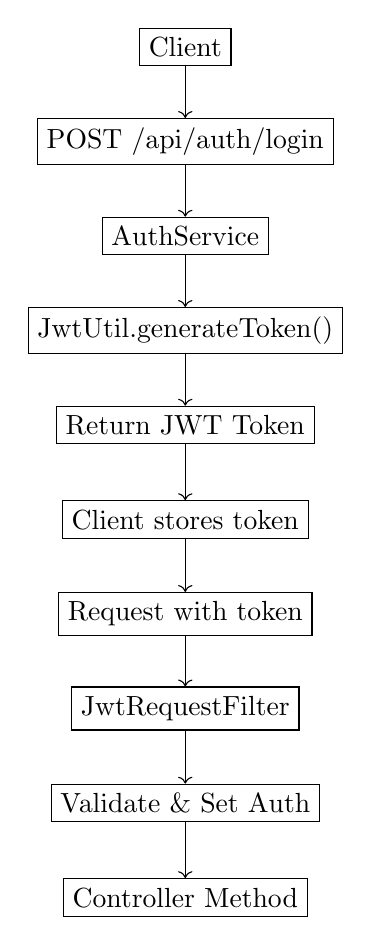
\begin{tikzpicture}[node distance=1.2cm]
    \node[draw, rectangle] (client) {Client};
    \node[draw, rectangle, below of=client] (login) {POST /api/auth/login};
    \node[draw, rectangle, below of=login] (authservice) {AuthService};
    \node[draw, rectangle, below of=authservice] (jwtutil) {JwtUtil.generateToken()};
    \node[draw, rectangle, below of=jwtutil] (response) {Return JWT Token};
    \node[draw, rectangle, below of=response] (store) {Client stores token};
    \node[draw, rectangle, below of=store] (request) {Request with token};
    \node[draw, rectangle, below of=request] (filter) {JwtRequestFilter};
    \node[draw, rectangle, below of=filter] (validate) {Validate \& Set Auth};
    \node[draw, rectangle, below of=validate] (controller) {Controller Method};
    
    \draw[->] (client) -- (login);
    \draw[->] (login) -- (authservice);
    \draw[->] (authservice) -- (jwtutil);
    \draw[->] (jwtutil) -- (response);
    \draw[->] (response) -- (store);
    \draw[->] (store) -- (request);
    \draw[->] (request) -- (filter);
    \draw[->] (filter) -- (validate);
    \draw[->] (validate) -- (controller);
\end{tikzpicture}
\caption{Complete Authentication Flow}
\end{figure}

\section{JWT Token Example}

\subsection{Token Structure}

A JWT consists of three parts separated by dots:

\texttt{header.payload.signature}

\textbf{Header (Base64):}
\begin{lstlisting}[language=json]
{
  ''alg'': ''HS512'',
  ''typ'': ''JWT''
}
\end{lstlisting}

\textbf{Payload (Base64):}
\begin{lstlisting}[language=json]
{
  ''role'': ''ADMIN'',
  ''sub'': ''admin@quizforge.com'',
  ''iat'': 1699632000,
  ''exp'': 1699718400
}
\end{lstlisting}

\textbf{Signature:}
\begin{lstlisting}
HMACSHA512(
  base64UrlEncode(header) + ''.'' + base64UrlEncode(payload),
  secret
)
\end{lstlisting}


% Chapter 8: API Documentation
\chapter{OpenAPI 3.0 Documentation}

\section{OpenAPI Configuration}

\subsection{OpenApiConfig Class}

\begin{lstlisting}[caption=OpenApiConfig.java]
@Configuration
public class OpenApiConfig {

    @Bean
    public OpenAPI customOpenAPI() {
        return new OpenAPI()
                .info(new Info()
                        .title(''QuizForge API'')
                        .version(''1.0'')
                        .description(''Online Quiz Platform - Role-based API (ADMIN & CANDIDATE)''))
                .servers(List.of(new Server()
                    .url(''http://localhost:8080'')
                    .description(''Development Server'')))
                .addSecurityItem(new SecurityRequirement()
                    .addList(''bearerAuth''))
                .components(new Components()
                        .addSecuritySchemes(''bearerAuth'',
                                new SecurityScheme()
                                        .type(SecurityScheme.Type.HTTP)
                                        .scheme(''bearer'')
                                        .bearerFormat(''JWT'')
                                        .description(''Enter JWT token obtained from /api/auth/login'')));
    }
}
\end{lstlisting}

\subsection{Configuration Elements}

\begin{itemize}
    \item \textbf{Info:} API metadata (title, version, description)
    \item \textbf{Servers:} Available server endpoints
    \item \textbf{SecurityRequirement:} Global security requirement
    \item \textbf{SecurityScheme:} JWT Bearer authentication definition
\end{itemize}

\section{API Endpoints Reference}

\subsection{Authentication Endpoints}

\begin{longtable}{|p{3cm}|p{10cm}|}
\hline
\textbf{Endpoint} & POST /api/auth/login \\
\hline
\textbf{Summary} & Login and get JWT token \\
\hline
\textbf{Description} & Use admin@quizforge.com for ADMIN role, any other email for CANDIDATE role \\
\hline
\textbf{Request Body} & \begin{lstlisting}[language=json]
{
  ''email'': ''string'',
  ''password'': ''string''
}
\end{lstlisting} \\
\hline
\textbf{Response 200} & \begin{lstlisting}[language=json]
{
  ''token'': ''string'',
  ''email'': ''string'',
  ''name'': ''string'',
  ''role'': ''string''
}
\end{lstlisting} \\
\hline
\textbf{Security} & None (public endpoint) \\
\hline
\caption{Login Endpoint Documentation}
\end{longtable}

\subsection{Admin Endpoints}

\subsubsection{GET /api/admin/quizzes}

\begin{longtable}{|p{3cm}|p{10cm}|}
\hline
\textbf{Summary} & Get all quizzes \\
\hline
\textbf{Description} & Retrieve list of all quizzes \\
\hline
\textbf{Security} & Bearer JWT (ADMIN role required) \\
\hline
\textbf{Response 200} & Array of QuizSummaryResponse \\
\hline
\textbf{Response Example} & \begin{lstlisting}[language=json]
[
  {
    ''id'': 1,
    ''title'': ''Java Basics'',
    ''description'': ''Test your Java knowledge'',
    ''duration'': 30,
    ''isActive'': true,
    ''createdBy'': ''Admin User'',
    ''createdAt'': ''2024-11-10T10:00:00'',
    ''questionCount'': 10
  }
]
\end{lstlisting} \\
\hline
\caption{Get All Quizzes Documentation}
\end{longtable}

\subsubsection{GET /api/admin/quizzes/\{id\}}

\begin{longtable}{|p{3cm}|p{10cm}|}
\hline
\textbf{Summary} & Get quiz by ID \\
\hline
\textbf{Parameters} & id (path, required): Quiz ID \\
\hline
\textbf{Security} & Bearer JWT (ADMIN role) \\
\hline
\textbf{Response 200} & QuizResponse with full details \\
\hline
\textbf{Response 404} & Quiz not found \\
\hline
\caption{Get Quiz by ID Documentation}
\end{longtable}

\subsubsection{POST /api/admin/quizzes}

\begin{longtable}{|p{3cm}|p{10cm}|}
\hline
\textbf{Summary} & Create new quiz \\
\hline
\textbf{Request Body} & \begin{lstlisting}[language=json, basicstyle=\ttfamily\tiny]
{
  ''title'': ''Java Basics'',
  ''description'': ''Test your Java knowledge'',
  ''duration'': 30,
  ''isActive'': true,
  ''questions'': [
    {
      ''questionText'': ''What is Java?'',
      ''type'': ''MULTIPLE_CHOICE'',
      ''points'': 1,
      ''options'': [
        {
          ''optionText'': ''Programming language'',
          ''isCorrect'': true
        },
        {
          ''optionText'': ''Coffee brand'',
          ''isCorrect'': false
        }
      ]
    }
  ]
}
\end{lstlisting} \\
\hline
\textbf{Response 201} & Created quiz with assigned IDs \\
\hline
\textbf{Response 400} & Validation errors \\
\hline
\caption{Create Quiz Documentation}
\end{longtable}

\subsubsection{PUT /api/admin/quizzes/\{id\}}

\begin{longtable}{|p{3cm}|p{10cm}|}
\hline
\textbf{Summary} & Update existing quiz \\
\hline
\textbf{Parameters} & id (path, required): Quiz ID \\
\hline
\textbf{Request Body} & Same as POST (full quiz data) \\
\hline
\textbf{Response 200} & Updated quiz \\
\hline
\textbf{Response 404} & Quiz not found \\
\hline
\caption{Update Quiz Documentation}
\end{longtable}

\subsubsection{DELETE /api/admin/quizzes/\{id\}}

\begin{longtable}{|p{3cm}|p{10cm}|}
\hline
\textbf{Summary} & Delete quiz \\
\hline
\textbf{Parameters} & id (path, required): Quiz ID \\
\hline
\textbf{Response 204} & No content (success) \\
\hline
\textbf{Response 404} & Quiz not found \\
\hline
\caption{Delete Quiz Documentation}
\end{longtable}

\subsubsection{GET /api/admin/quizzes/\{id\}/analytics}

\begin{longtable}{|p{3cm}|p{10cm}|}
\hline
\textbf{Summary} & Get quiz analytics \\
\hline
\textbf{Parameters} & id (path, required): Quiz ID \\
\hline
\textbf{Response 200} & \begin{lstlisting}[language=json]
{
  ''quizId'': 1,
  ''quizTitle'': ''Java Basics'',
  ''totalAttempts'': 15,
  ''averageScore'': 7.5,
  ''highestScore'': 10,
  ''lowestScore'': 3
}
\end{lstlisting} \\
\hline
\caption{Quiz Analytics Documentation}
\end{longtable}

\subsection{Candidate Endpoints}

\subsubsection{GET /api/candidate/quizzes}

\begin{longtable}{|p{3cm}|p{10cm}|}
\hline
\textbf{Summary} & Get available quizzes \\
\hline
\textbf{Security} & Bearer JWT (CANDIDATE role) \\
\hline
\textbf{Response 200} & Array of active quizzes (summary) \\
\hline
\caption{Get Available Quizzes Documentation}
\end{longtable}

\subsubsection{POST /api/candidate/quizzes/\{quizId\}/start}

\begin{longtable}{|p{3cm}|p{10cm}|}
\hline
\textbf{Summary} & Start quiz attempt \\
\hline
\textbf{Parameters} & quizId (path, required) \\
\hline
\textbf{Response 200} & \begin{lstlisting}[language=json]
{
  ''id'': 1,
  ''quizId'': 1,
  ''quizTitle'': ''Java Basics'',
  ''startedAt'': ''2024-11-10T10:00:00'',
  ''submittedAt'': null,
  ''score'': null,
  ''totalPoints'': 10,
  ''status'': ''IN_PROGRESS''
}
\end{lstlisting} \\
\hline
\caption{Start Quiz Documentation}
\end{longtable}

\subsubsection{GET /api/candidate/quizzes/\{quizId\}}

\begin{longtable}{|p{3cm}|p{10cm}|}
\hline
\textbf{Summary} & Get quiz questions \\
\hline
\textbf{Description} & Returns questions with options, but isCorrect is hidden \\
\hline
\textbf{Parameters} & quizId (path, required) \\
\hline
\textbf{Response 200} & QuizResponse (without correct answers) \\
\hline
\caption{Get Quiz Questions Documentation}
\end{longtable}

\subsubsection{POST /api/candidate/quizzes/submit}

\begin{longtable}{|p{3cm}|p{10cm}|}
\hline
\textbf{Summary} & Submit quiz answers \\
\hline
\textbf{Request Body} & \begin{lstlisting}[language=json]
{
  ''attemptId'': 1,
  ''answers'': [
    {
      ''questionId'': 1,
      ''selectedOptionId'': 3,
      ''textAnswer'': null
    },
    {
      ''questionId'': 2,
      ''selectedOptionId'': null,
      ''textAnswer'': ''Sample answer''
    }
  ]
}
\end{lstlisting} \\
\hline
\textbf{Response 200} & AttemptResponse with calculated score \\
\hline
\caption{Submit Quiz Documentation}
\end{longtable}

\subsubsection{GET /api/candidate/quizzes/my-attempts}

\begin{longtable}{|p{3cm}|p{10cm}|}
\hline
\textbf{Summary} & Get my quiz attempts \\
\hline
\textbf{Response 200} & Array of user's attempts with scores \\
\hline
\caption{Get My Attempts Documentation}
\end{longtable}

\subsubsection{GET /api/candidate/quizzes/attempts/\{attemptId\}}

\begin{longtable}{|p{3cm}|p{10cm}|}
\hline
\textbf{Summary} & Get attempt result \\
\hline
\textbf{Parameters} & attemptId (path, required) \\
\hline
\textbf{Response 200} & Detailed attempt results \\
\hline
\textbf{Response 403} & Not your attempt (forbidden) \\
\hline
\caption{Get Attempt Result Documentation}
\end{longtable}

\section{Swagger UI Access}

The interactive API documentation is available at:

\texttt{http://localhost:8080/swagger-ui.html}

Features:
\begin{itemize}
    \item Try API endpoints directly from browser
    \item Automatic request/response examples
    \item JWT authentication support
    \item Grouped by controller tags
    \item Alphabetically sorted operations
\end{itemize}

\section{OpenAPI JSON Specification}

The raw OpenAPI 3.0 specification is available at:

\texttt{http://localhost:8080/v3/api-docs}

Can be used with:
\begin{itemize}
    \item Code generators (OpenAPI Generator)
    \item API testing tools (Postman, Insomnia)
    \item Documentation generators
    \item Mock server tools
\end{itemize}


% Chapter 9: ER Diagram
\chapter{Entity-Relationship Diagram}

\section{Complete ER Diagram}

\begin{landscape}
\begin{figure}[h]
\centering
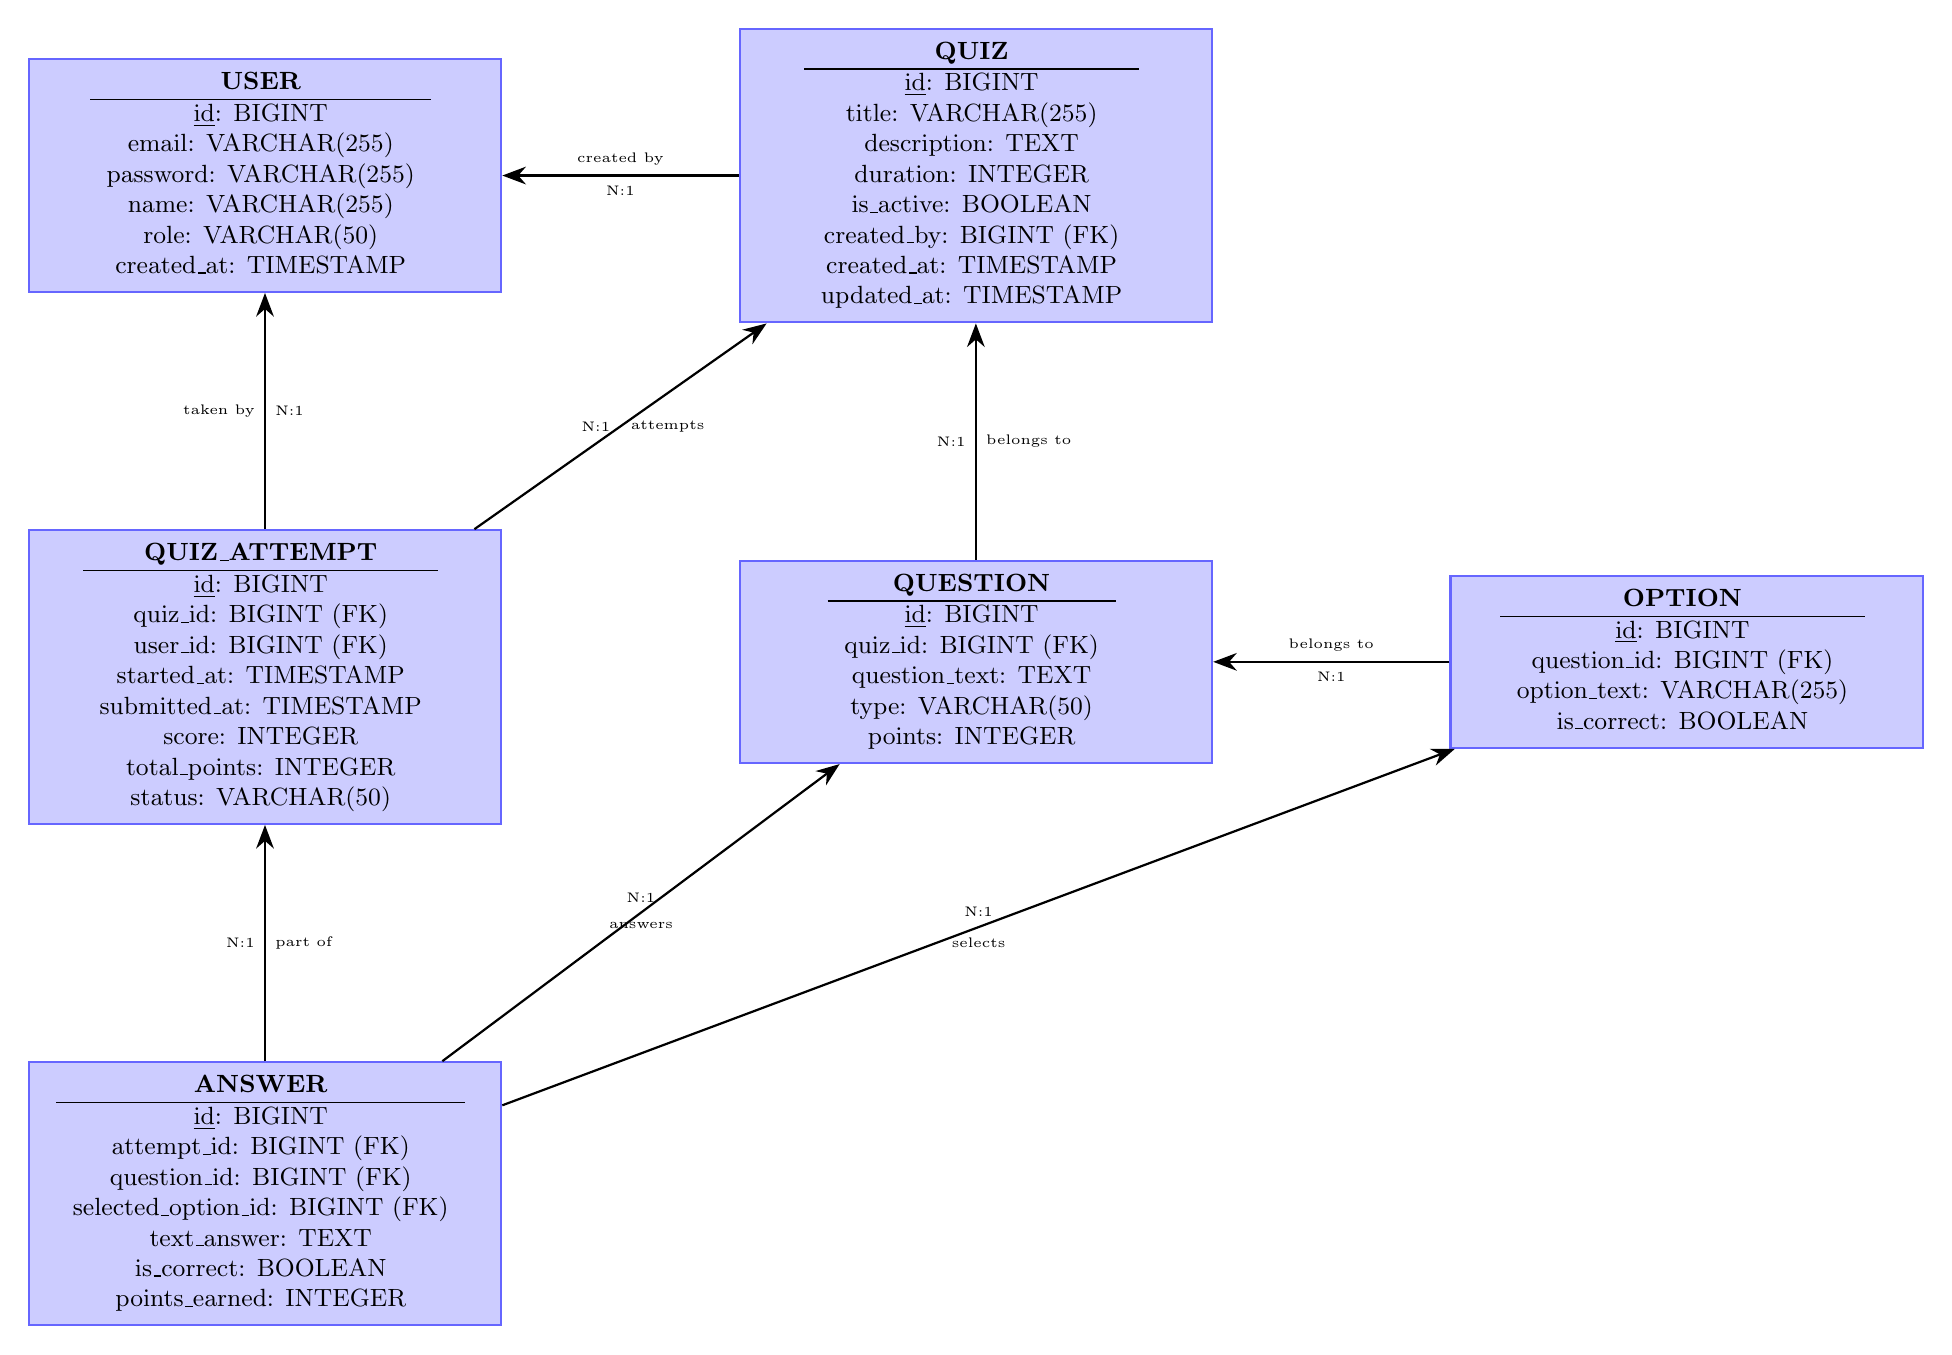
\begin{tikzpicture}[
    node distance=3cm,
    entity/.style={rectangle, draw=blue!60, fill=blue!20, thick, minimum width=6cm, align=center},
    relationship/.style={-{Stealth[length=3mm]}, thick},
    every node/.style={font=\small}
]
    
    % User Entity
    \node[entity] (user) {
        \begin{tabular}{c}
            \textbf{USER} \\
            \hline
            \underline{id}: BIGINT \\
            email: VARCHAR(255) \\
            password: VARCHAR(255) \\
            name: VARCHAR(255) \\
            role: VARCHAR(50) \\
            created\_at: TIMESTAMP
        \end{tabular}
    };
    
    % Quiz Entity
    \node[entity, right=of user] (quiz) {
        \begin{tabular}{c}
            \textbf{QUIZ} \\
            \hline
            \underline{id}: BIGINT \\
            title: VARCHAR(255) \\
            description: TEXT \\
            duration: INTEGER \\
            is\_active: BOOLEAN \\
            created\_by: BIGINT (FK) \\
            created\_at: TIMESTAMP \\
            updated\_at: TIMESTAMP
        \end{tabular}
    };
    
    % Question Entity
    \node[entity, below=of quiz] (question) {
        \begin{tabular}{c}
            \textbf{QUESTION} \\
            \hline
            \underline{id}: BIGINT \\
            quiz\_id: BIGINT (FK) \\
            question\_text: TEXT \\
            type: VARCHAR(50) \\
            points: INTEGER
        \end{tabular}
    };
    
    % Option Entity
    \node[entity, right=of question] (option) {
        \begin{tabular}{c}
            \textbf{OPTION} \\
            \hline
            \underline{id}: BIGINT \\
            question\_id: BIGINT (FK) \\
            option\_text: VARCHAR(255) \\
            is\_correct: BOOLEAN
        \end{tabular}
    };
    
    % QuizAttempt Entity
    \node[entity, below=of user] (attempt) {
        \begin{tabular}{c}
            \textbf{QUIZ\_ATTEMPT} \\
            \hline
            \underline{id}: BIGINT \\
            quiz\_id: BIGINT (FK) \\
            user\_id: BIGINT (FK) \\
            started\_at: TIMESTAMP \\
            submitted\_at: TIMESTAMP \\
            score: INTEGER \\
            total\_points: INTEGER \\
            status: VARCHAR(50)
        \end{tabular}
    };
    
    % Answer Entity
    \node[entity, below=of attempt] (answer) {
        \begin{tabular}{c}
            \textbf{ANSWER} \\
            \hline
            \underline{id}: BIGINT \\
            attempt\_id: BIGINT (FK) \\
            question\_id: BIGINT (FK) \\
            selected\_option\_id: BIGINT (FK) \\
            text\_answer: TEXT \\
            is\_correct: BOOLEAN \\
            points\_earned: INTEGER
        \end{tabular}
    };
    
    % Relationships
    \draw[relationship] (quiz) -- (user) node[midway, above, font=\tiny] {created by} node[midway, below, font=\tiny] {N:1};
    \draw[relationship] (question) -- (quiz) node[midway, right, font=\tiny] {belongs to} node[midway, left, font=\tiny] {N:1};
    \draw[relationship] (option) -- (question) node[midway, above, font=\tiny] {belongs to} node[midway, below, font=\tiny] {N:1};
    \draw[relationship] (attempt) -- (quiz) node[midway, right, font=\tiny] {attempts} node[midway, left, font=\tiny] {N:1};
    \draw[relationship] (attempt) -- (user) node[midway, left, font=\tiny] {taken by} node[midway, right, font=\tiny] {N:1};
    \draw[relationship] (answer) -- (attempt) node[midway, right, font=\tiny] {part of} node[midway, left, font=\tiny] {N:1};
    \draw[relationship] (answer) -- (question) node[midway, below, font=\tiny] {answers} node[midway, above, font=\tiny] {N:1};
    \draw[relationship] (answer) -- (option) node[midway, below, font=\tiny] {selects} node[midway, above, font=\tiny] {N:1};
    
\end{tikzpicture}
\caption{Complete Entity-Relationship Diagram}
\end{figure}
\end{landscape}

\section{Relationship Details}

\subsection{User $\rightarrow$ Quiz (created\_by)}

\begin{table}[h]
\centering
\begin{tabular}{|l|p{8cm}|}
\hline
\textbf{Type} & One-to-Many \\
\hline
\textbf{Cardinality} & 1 User : N Quizzes \\
\hline
\textbf{Direction} & Unidirectional (Quiz $\rightarrow$ User) \\
\hline
\textbf{Foreign Key} & quizzes.created\_by $\rightarrow$ users.id \\
\hline
\textbf{On Delete} & Depends on business rule (typically RESTRICT) \\
\hline
\textbf{Description} & Each quiz is created by exactly one admin user. A user (admin) can create multiple quizzes. \\
\hline
\textbf{JPA Mapping} & @ManyToOne(fetch = FetchType.LAZY) in Quiz \\
\hline
\end{tabular}
\caption{User-Quiz Relationship}
\end{table}

\textbf{SQL Constraint:}
\begin{lstlisting}[language=SQL]
ALTER TABLE quizzes
ADD CONSTRAINT fk_quiz_created_by
FOREIGN KEY (created_by) REFERENCES users(id);
\end{lstlisting}

\subsection{Quiz $\leftrightarrow$ Question}

\begin{table}[h]
\centering
\begin{tabular}{|l|p{8cm}|}
\hline
\textbf{Type} & One-to-Many (Bidirectional) \\
\hline
\textbf{Cardinality} & 1 Quiz : N Questions \\
\hline
\textbf{Foreign Key} & questions.quiz\_id $\rightarrow$ quizzes.id \\
\hline
\textbf{Cascade} & ALL (persist, merge, remove, refresh, detach) \\
\hline
\textbf{Orphan Removal} & true (delete questions if removed from list) \\
\hline
\textbf{Description} & Each question belongs to exactly one quiz. A quiz contains multiple questions. When a quiz is deleted, all its questions are automatically deleted. \\
\hline
\textbf{JPA Mapping} & @OneToMany in Quiz, @ManyToOne in Question \\
\hline
\end{tabular}
\caption{Quiz-Question Relationship}
\end{table}

\textbf{SQL Constraint:}
\begin{lstlisting}[language=SQL]
ALTER TABLE questions
ADD CONSTRAINT fk_question_quiz
FOREIGN KEY (quiz_id) REFERENCES quizzes(id)
ON DELETE CASCADE;
\end{lstlisting}

\subsection{Question $\leftrightarrow$ Option}

\begin{table}[h]
\centering
\begin{tabular}{|l|p{8cm}|}
\hline
\textbf{Type} & One-to-Many (Bidirectional) \\
\hline
\textbf{Cardinality} & 1 Question : N Options \\
\hline
\textbf{Foreign Key} & options.question\_id $\rightarrow$ questions.id \\
\hline
\textbf{Cascade} & ALL \\
\hline
\textbf{Orphan Removal} & true \\
\hline
\textbf{Description} & Each option belongs to exactly one question. A question can have multiple options (typically 4-5 for multiple choice). Options are deleted when question is deleted. \\
\hline
\textbf{JPA Mapping} & @OneToMany in Question, @ManyToOne in Option \\
\hline
\end{tabular}
\caption{Question-Option Relationship}
\end{table}

\subsection{Quiz $\rightarrow$ QuizAttempt}

\begin{table}[h]
\centering
\begin{tabular}{|l|p{8cm}|}
\hline
\textbf{Type} & One-to-Many \\
\hline
\textbf{Cardinality} & 1 Quiz : N Attempts \\
\hline
\textbf{Foreign Key} & quiz\_attempts.quiz\_id $\rightarrow$ quizzes.id \\
\hline
\textbf{Description} & Each attempt is for exactly one quiz. A quiz can have multiple attempts from different candidates. \\
\hline
\textbf{Business Rule} & Typically prevent quiz deletion if attempts exist \\
\hline
\end{tabular}
\caption{Quiz-Attempt Relationship}
\end{table}

\subsection{User $\rightarrow$ QuizAttempt}

\begin{table}[h]
\centering
\begin{tabular}{|l|p{8cm}|}
\hline
\textbf{Type} & One-to-Many \\
\hline
\textbf{Cardinality} & 1 User : N Attempts \\
\hline
\textbf{Foreign Key} & quiz\_attempts.user\_id $\rightarrow$ users.id \\
\hline
\textbf{Description} & Each attempt is taken by exactly one candidate. A candidate can take multiple quizzes and can retake the same quiz multiple times. \\
\hline
\end{tabular}
\caption{User-Attempt Relationship}
\end{table}

\subsection{QuizAttempt $\leftrightarrow$ Answer}

\begin{table}[h]
\centering
\begin{tabular}{|l|p{8cm}|}
\hline
\textbf{Type} & One-to-Many (Bidirectional) \\
\hline
\textbf{Cardinality} & 1 Attempt : N Answers \\
\hline
\textbf{Foreign Key} & answers.attempt\_id $\rightarrow$ quiz\_attempts.id \\
\hline
\textbf{Cascade} & ALL \\
\hline
\textbf{Orphan Removal} & true \\
\hline
\textbf{Description} & Each answer belongs to exactly one attempt. An attempt contains multiple answers (one per question). Answers are deleted when attempt is deleted. \\
\hline
\end{tabular}
\caption{Attempt-Answer Relationship}
\end{table}

\subsection{Question $\rightarrow$ Answer}

\begin{table}[h]
\centering
\begin{tabular}{|l|p{8cm}|}
\hline
\textbf{Type} & One-to-Many \\
\hline
\textbf{Cardinality} & 1 Question : N Answers \\
\hline
\textbf{Foreign Key} & answers.question\_id $\rightarrow$ questions.id \\
\hline
\textbf{Description} & Each answer is for exactly one question. A question can have many answers across different attempts. \\
\hline
\end{tabular}
\caption{Question-Answer Relationship}
\end{table}

\subsection{Option $\rightarrow$ Answer}

\begin{table}[h]
\centering
\begin{tabular}{|l|p{8cm}|}
\hline
\textbf{Type} & One-to-Many (Optional) \\
\hline
\textbf{Cardinality} & 1 Option : N Answers \\
\hline
\textbf{Foreign Key} & answers.selected\_option\_id $\rightarrow$ options.id (NULLABLE) \\
\hline
\textbf{Description} & For multiple-choice questions, an answer references the selected option. For short-answer questions, this field is null. An option can be selected by multiple candidates. \\
\hline
\end{tabular}
\caption{Option-Answer Relationship}
\end{table}

\section{Database Constraints}

\subsection{Primary Keys}

All tables use auto-incrementing BIGINT primary keys:
\begin{itemize}
    \item BIGSERIAL in PostgreSQL
    \item GenerationType.IDENTITY in JPA
    \item Range: -9,223,372,036,854,775,808 to 9,223,372,036,854,775,807
\end{itemize}

\subsection{Foreign Key Constraints}

\begin{table}[h]
\centering
\small
\begin{tabular}{|l|l|l|}
\hline
\textbf{Table} & \textbf{FK Column} & \textbf{References} \\
\hline
quizzes & created\_by & users(id) \\
\hline
questions & quiz\_id & quizzes(id) \\
\hline
options & question\_id & questions(id) \\
\hline
quiz\_attempts & quiz\_id & quizzes(id) \\
\hline
quiz\_attempts & user\_id & users(id) \\
\hline
answers & attempt\_id & quiz\_attempts(id) \\
\hline
answers & question\_id & questions(id) \\
\hline
answers & selected\_option\_id & options(id) \\
\hline
\end{tabular}
\caption{Foreign Key Summary}
\end{table}

\subsection{Unique Constraints}

\begin{itemize}
    \item \textbf{users.email}: Must be unique (used for authentication)
\end{itemize}

\subsection{Not Null Constraints}

Critical fields that cannot be null:
\begin{itemize}
    \item All primary keys
    \item All foreign keys (except answers.selected\_option\_id)
    \item users: email, password, name, role, created\_at
    \item quizzes: title, duration, is\_active, created\_by
    \item questions: quiz\_id, question\_text, type, points
    \item options: question\_id, option\_text, is\_correct
    \item quiz\_attempts: quiz\_id, user\_id, started\_at, status
    \item answers: attempt\_id, question\_id, is\_correct
\end{itemize}

\section{Indexes}

Recommended indexes for performance:

\begin{lstlisting}[language=SQL]
-- Email lookup for authentication
CREATE INDEX idx_users_email ON users(email);

-- Active quiz queries
CREATE INDEX idx_quizzes_is_active ON quizzes(is_active);

-- User attempt history
CREATE INDEX idx_quiz_attempts_user_id ON quiz_attempts(user_id);

-- Quiz analytics
CREATE INDEX idx_quiz_attempts_quiz_id ON quiz_attempts(quiz_id);

-- Attempt status filtering
CREATE INDEX idx_quiz_attempts_status ON quiz_attempts(status);
\end{lstlisting}


% Chapter 10: Configuration
\chapter{Application Configuration}

\section{application.properties}

\subsection{Complete Configuration File}

\begin{lstlisting}[caption=application.properties]
# Server Configuration
server.port=8080

# Database Configuration
spring.datasource.url=jdbc:postgresql://localhost:5432/quizforge_db
spring.datasource.username=quizforge_user
spring.datasource.password=quizforge_pass
spring.datasource.driver-class-name=org.postgresql.Driver

# JPA Configuration
spring.jpa.hibernate.ddl-auto=update
spring.jpa.show-sql=true
spring.jpa.properties.hibernate.dialect=org.hibernate.dialect.PostgreSQLDialect
spring.jpa.properties.hibernate.format_sql=true

# JWT Configuration
jwt.secret=YourSuperSecretKeyForJWTTokenGenerationMustBeLongEnoughForHS512Algorithm
jwt.expiration=86400000

# Swagger/OpenAPI Configuration
springdoc.api-docs.enabled=true
springdoc.swagger-ui.enabled=true
springdoc.api-docs.path=/v3/api-docs
springdoc.swagger-ui.path=/swagger-ui.html
springdoc.swagger-ui.operationsSorter=method
springdoc.swagger-ui.tagsSorter=alpha
springdoc.swagger-ui.disable-swagger-default-url=true

# CORS Configuration
cors.allowed-origins=http://localhost:5173
\end{lstlisting}

\section{Configuration Sections Explained}

\subsection{Server Configuration}

\begin{table}[h]
\centering
\begin{tabular}{|l|l|p{6cm}|}
\hline
\textbf{Property} & \textbf{Value} & \textbf{Description} \\
\hline
server.port & 8080 & HTTP port for application \\
\hline
\end{tabular}
\caption{Server Configuration}
\end{table}

\textbf{Notes:}
\begin{itemize}
    \item Default Spring Boot port
    \item Can be changed for multiple instances
    \item Use environment variable: \texttt{SERVER\_PORT=9090}
\end{itemize}

\subsection{Database Configuration}

\begin{table}[h]
\centering
\small
\begin{tabular}{|l|p{10cm}|}
\hline
\textbf{Property} & \textbf{Description} \\
\hline
spring.datasource.url & JDBC URL for PostgreSQL database. Format: jdbc:postgresql://host:port/database \\
\hline
spring.datasource.username & Database user with appropriate permissions \\
\hline
spring.datasource.password & Database password (should be externalized in production) \\
\hline
spring.datasource.driver-class-name & PostgreSQL JDBC driver class \\
\hline
\end{tabular}
\caption{Database Configuration}
\end{table}

\textbf{Database Setup Script:}
\begin{lstlisting}[language=bash]
# Create database and user
sudo -u postgres psql
CREATE DATABASE quizforge_db;
CREATE USER quizforge_user WITH PASSWORD 'quizforge_pass';
GRANT ALL PRIVILEGES ON DATABASE quizforge_db TO quizforge_user;
\end{lstlisting}

\subsection{JPA Configuration}

\begin{table}[h]
\centering
\small
\begin{tabular}{|l|p{8cm}|}
\hline
\textbf{Property} & \textbf{Description} \\
\hline
spring.jpa.hibernate.ddl-auto & \textbf{update}: Automatically update schema based on entities. Options: none, validate, update, create, create-drop \\
\hline
spring.jpa.show-sql & \textbf{true}: Log SQL queries to console (useful for development) \\
\hline
spring.jpa.properties.hibernate.dialect & PostgreSQL-specific SQL dialect \\
\hline
spring.jpa.properties.hibernate.format\_sql & \textbf{true}: Pretty-print SQL for readability \\
\hline
\end{tabular}
\caption{JPA Configuration}
\end{table}

\textbf{DDL-Auto Options:}
\begin{itemize}
    \item \textbf{none}: No schema management
    \item \textbf{validate}: Validate schema matches entities (production)
    \item \textbf{update}: Update schema (development)
    \item \textbf{create}: Drop and recreate schema (testing)
    \item \textbf{create-drop}: Drop schema on shutdown (testing)
\end{itemize}

\textbf{Production Recommendation:}
\begin{lstlisting}
spring.jpa.hibernate.ddl-auto=validate
spring.jpa.show-sql=false
\end{lstlisting}

\subsection{JWT Configuration}

\begin{table}[h]
\centering
\begin{tabular}{|l|p{8cm}|}
\hline
\textbf{Property} & \textbf{Description} \\
\hline
jwt.secret & Secret key for signing JWT tokens. Must be long enough for HS512 (at least 512 bits / 64 bytes). Should be stored securely in production. \\
\hline
jwt.expiration & Token expiration time in milliseconds. 86400000 ms = 24 hours. \\
\hline
\end{tabular}
\caption{JWT Configuration}
\end{table}

\textbf{Security Best Practices:}
\begin{itemize}
    \item Generate strong random secret: \texttt{openssl rand -base64 64}
    \item Store in environment variable or secret manager
    \item Rotate secrets periodically
    \item Use different secrets for different environments
\end{itemize}

\textbf{Expiration Time Examples:}
\begin{lstlisting}
15 minutes  = 900000
1 hour      = 3600000
24 hours    = 86400000
7 days      = 604800000
\end{lstlisting}

\subsection{Swagger/OpenAPI Configuration}

\begin{table}[h]
\centering
\small
\begin{tabular}{|l|p{8cm}|}
\hline
\textbf{Property} & \textbf{Description} \\
\hline
springdoc.api-docs.enabled & Enable OpenAPI JSON generation \\
\hline
springdoc.swagger-ui.enabled & Enable Swagger UI web interface \\
\hline
springdoc.api-docs.path & URL path for OpenAPI JSON \\
\hline
springdoc.swagger-ui.path & URL path for Swagger UI \\
\hline
springdoc.swagger-ui.operationsSorter & Sort operations by HTTP method \\
\hline
springdoc.swagger-ui.tagsSorter & Sort tags alphabetically \\
\hline
springdoc.swagger-ui.disable-swagger-default-url & Disable default Swagger URL \\
\hline
\end{tabular}
\caption{Swagger Configuration}
\end{table}

\textbf{Access URLs:}
\begin{itemize}
    \item Swagger UI: \texttt{http://localhost:8080/swagger-ui.html}
    \item OpenAPI JSON: \texttt{http://localhost:8080/v3/api-docs}
\end{itemize}

\textbf{Production Consideration:}
Disable Swagger in production or protect with authentication:
\begin{lstlisting}
springdoc.swagger-ui.enabled=false  # Production
\end{lstlisting}

\subsection{CORS Configuration}

\begin{table}[h]
\centering
\begin{tabular}{|l|p{8cm}|}
\hline
\textbf{Property} & \textbf{Description} \\
\hline
cors.allowed-origins & Comma-separated list of allowed origin URLs for CORS. Frontend application URL. \\
\hline
\end{tabular}
\caption{CORS Configuration}
\end{table}

\textbf{Multiple Origins Example:}
\begin{lstlisting}
cors.allowed-origins=http://localhost:5173,http://localhost:3000,https://quizforge.com
\end{lstlisting}

\section{Maven Configuration (pom.xml)}

\subsection{Project Information}

\begin{lstlisting}[language=XML]
<groupId>com.quizforge</groupId>
<artifactId>quizforge</artifactId>
<version>1.0.0</version>
<name>QuizForge</name>
<description>Online Quiz Platform</description>
\end{lstlisting}

\subsection{Java Version}

\begin{lstlisting}[language=XML]
<properties>
    <java.version>21</java.version>
    <springdoc.version>2.6.0</springdoc.version>
</properties>
\end{lstlisting}

\textbf{Java 21 Features Used:}
\begin{itemize}
    \item Record classes (DTOs)
    \item Pattern matching
    \item Switch expressions
    \item Text blocks
    \item Improved garbage collection
\end{itemize}

\subsection{Parent POM}

\begin{lstlisting}[language=XML]
<parent>
    <groupId>org.springframework.boot</groupId>
    <artifactId>spring-boot-starter-parent</artifactId>
    <version>3.2.0</version>
    <relativePath/>
</parent>
\end{lstlisting}

Benefits:
\begin{itemize}
    \item Dependency management
    \item Default plugin configuration
    \item Common Spring Boot defaults
\end{itemize}

\section{Environment-Specific Configuration}

\subsection{Profile-Based Configuration}

Spring supports multiple profiles:

\textbf{application-dev.properties:}
\begin{lstlisting}
spring.jpa.show-sql=true
spring.jpa.hibernate.ddl-auto=update
\end{lstlisting}

\textbf{application-prod.properties:}
\begin{lstlisting}
spring.jpa.show-sql=false
spring.jpa.hibernate.ddl-auto=validate
springdoc.swagger-ui.enabled=false
\end{lstlisting}

\textbf{Activation:}
\begin{lstlisting}[language=bash]
# Command line
java -jar app.jar --spring.profiles.active=prod

# Environment variable
export SPRING_PROFILES_ACTIVE=prod
\end{lstlisting}

\subsection{External Configuration}

For production, externalize sensitive configuration:

\textbf{Using Environment Variables:}
\begin{lstlisting}
spring.datasource.url=${DB_URL}
spring.datasource.username=${DB_USERNAME}
spring.datasource.password=${DB_PASSWORD}
jwt.secret=${JWT_SECRET}
\end{lstlisting}

\textbf{Using External application.properties:}
\begin{lstlisting}[language=bash]
java -jar app.jar --spring.config.location=/etc/quizforge/application.properties
\end{lstlisting}

\section{Database Migration Tools}

For production, consider using migration tools:

\subsection{Flyway Configuration}

\begin{lstlisting}[language=XML]
<dependency>
    <groupId>org.flywaydb</groupId>
    <artifactId>flyway-core</artifactId>
</dependency>
\end{lstlisting}

\begin{lstlisting}
spring.flyway.enabled=true
spring.flyway.locations=classpath:db/migration
\end{lstlisting}

\subsection{Liquibase Configuration}

\begin{lstlisting}[language=XML]
<dependency>
    <groupId>org.liquibase</groupId>
    <artifactId>liquibase-core</artifactId>
</dependency>
\end{lstlisting}

\begin{lstlisting}
spring.liquibase.change-log=classpath:db/changelog/db.changelog-master.xml
\end{lstlisting}

\section{Logging Configuration}

\subsection{Logging Levels}

\begin{lstlisting}
# Root logging level
logging.level.root=INFO

# Package-specific logging
logging.level.com.quizforge=DEBUG
logging.level.org.springframework.security=DEBUG
logging.level.org.hibernate.SQL=DEBUG
logging.level.org.hibernate.type.descriptor.sql.BasicBinder=TRACE

# Log to file
logging.file.name=logs/quizforge.log
logging.file.max-size=10MB
logging.file.max-history=30
\end{lstlisting}

\subsection{Log Format}

\begin{lstlisting}
logging.pattern.console=%d{yyyy-MM-dd HH:mm:ss} - %msg%n
logging.pattern.file=%d{yyyy-MM-dd HH:mm:ss} [%thread] %-5level %logger{36} - %msg%n
\end{lstlisting}



% Appendix
\appendix
% Appendix A: Dependencies
\chapter{Complete Dependency List}

\section{Core Spring Boot Dependencies}

\subsection{Spring Boot Starter Web}

\begin{lstlisting}[language=XML]
<dependency>
    <groupId>org.springframework.boot</groupId>
    <artifactId>spring-boot-starter-web</artifactId>
</dependency>
\end{lstlisting}

\textbf{Includes:}
\begin{itemize}
    \item Spring MVC for REST APIs
    \item Embedded Tomcat server
    \item Jackson for JSON serialization
    \item Spring Web utilities
\end{itemize}

\subsection{Spring Boot Starter Security}

\begin{lstlisting}[language=XML]
<dependency>
    <groupId>org.springframework.boot</groupId>
    <artifactId>spring-boot-starter-security</artifactId>
</dependency>
\end{lstlisting}

\textbf{Includes:}
\begin{itemize}
    \item Spring Security Core
    \item Authentication mechanisms
    \item Authorization framework
    \item CSRF protection
    \item Security filters
\end{itemize}

\subsection{Spring Boot Starter Data JPA}

\begin{lstlisting}[language=XML]
<dependency>
    <groupId>org.springframework.boot</groupId>
    <artifactId>spring-boot-starter-data-jpa</artifactId>
</dependency>
\end{lstlisting}

\textbf{Includes:}
\begin{itemize}
    \item Hibernate ORM
    \item Spring Data JPA
    \item Jakarta Persistence API
    \item Connection pooling (HikariCP)
    \item Transaction management
\end{itemize}

\subsection{Spring Boot Starter Validation}

\begin{lstlisting}[language=XML]
<dependency>
    <groupId>org.springframework.boot</groupId>
    <artifactId>spring-boot-starter-validation</artifactId>
</dependency>
\end{lstlisting}

\textbf{Includes:}
\begin{itemize}
    \item Jakarta Bean Validation API
    \item Hibernate Validator implementation
    \item Annotations: @NotNull, @NotBlank, @Email, @Min, @Max, etc.
\end{itemize}

\section{JWT Dependencies}

\subsection{JJWT API}

\begin{lstlisting}[language=XML]
<dependency>
    <groupId>io.jsonwebtoken</groupId>
    <artifactId>jjwt-api</artifactId>
    <version>0.11.5</version>
</dependency>
\end{lstlisting}

\textbf{Purpose:} JWT token creation and parsing API

\subsection{JJWT Implementation}

\begin{lstlisting}[language=XML]
<dependency>
    <groupId>io.jsonwebtoken</groupId>
    <artifactId>jjwt-impl</artifactId>
    <version>0.11.5</version>
    <scope>runtime</scope>
</dependency>
\end{lstlisting}

\textbf{Purpose:} Runtime implementation of JJWT

\subsection{JJWT Jackson Integration}

\begin{lstlisting}[language=XML]
<dependency>
    <groupId>io.jsonwebtoken</groupId>
    <artifactId>jjwt-jackson</artifactId>
    <version>0.11.5</version>
    <scope>runtime</scope>
</dependency>
\end{lstlisting}

\textbf{Purpose:} JSON serialization for JWT claims

\section{Database Dependencies}

\subsection{PostgreSQL JDBC Driver}

\begin{lstlisting}[language=XML]
<dependency>
    <groupId>org.postgresql</groupId>
    <artifactId>postgresql</artifactId>
    <scope>runtime</scope>
</dependency>
\end{lstlisting}

\textbf{Version:} Managed by Spring Boot (42.x)

\textbf{Purpose:}
\begin{itemize}
    \item JDBC connection to PostgreSQL
    \item Type mappings
    \item PostgreSQL-specific features
\end{itemize}

\section{Documentation Dependencies}

\subsection{SpringDoc OpenAPI}

\begin{lstlisting}[language=XML]
<dependency>
    <groupId>org.springdoc</groupId>
    <artifactId>springdoc-openapi-starter-webmvc-ui</artifactId>
    <version>2.6.0</version>
</dependency>
\end{lstlisting}

\textbf{Features:}
\begin{itemize}
    \item OpenAPI 3.0 specification generation
    \item Swagger UI integration
    \item Automatic API documentation
    \item Interactive API testing
\end{itemize}

\textbf{Annotations Used:}
\begin{itemize}
    \item @Tag - Controller grouping
    \item @Operation - Endpoint documentation
    \item @SecurityRequirement - Auth requirements
    \item @Schema - DTO documentation
\end{itemize}

\section{Utility Dependencies}

\subsection{Lombok}

\begin{lstlisting}[language=XML]
<dependency>
    <groupId>org.projectlombok</groupId>
    <artifactId>lombok</artifactId>
    <optional>true</optional>
</dependency>
\end{lstlisting}

\textbf{Annotations Used:}
\begin{itemize}
    \item @Data - Generates getters, setters, toString, equals, hashCode
    \item @NoArgsConstructor - No-argument constructor
    \item @AllArgsConstructor - All-arguments constructor
    \item @Builder - Builder pattern
    \item @Slf4j - Logger instance
\end{itemize}

\textbf{IDE Setup Required:}
\begin{itemize}
    \item IntelliJ IDEA: Install Lombok plugin
    \item Eclipse: Run lombok.jar installer
    \item VS Code: Install Lombok extension
\end{itemize}

\section{Development Dependencies}

\subsection{Spring Boot DevTools}

\begin{lstlisting}[language=XML]
<dependency>
    <groupId>org.springframework.boot</groupId>
    <artifactId>spring-boot-devtools</artifactId>
    <scope>runtime</scope>
    <optional>true</optional>
</dependency>
\end{lstlisting}

\textbf{Features:}
\begin{itemize}
    \item Automatic application restart on code changes
    \item LiveReload browser integration
    \item Development-time property defaults
    \item Faster development cycle
\end{itemize}

\textbf{Note:} Not included in production builds

\section{Dependency Tree}

\subsection{Complete Dependency Hierarchy}

\begin{verbatim}
quizforge:1.0.0
|------ spring-boot-starter-web:3.2.0
|   |------ spring-boot-starter-json:3.2.0
|   |   \`------ jackson-databind:2.15.3
|   |------ spring-boot-starter-tomcat:3.2.0
|   \`------ spring-web:6.1.0
|       \`------ spring-webmvc:6.1.0
|------ spring-boot-starter-security:3.2.0
|   \`------ spring-security-web:6.2.0
|       \`------ spring-security-core:6.2.0
|------ spring-boot-starter-data-jpa:3.2.0
|   |------ hibernate-core:6.3.1
|   |------ spring-data-jpa:3.2.0
|   \`------ HikariCP:5.0.1
|------ postgresql:42.6.0
|------ jjwt-api:0.11.5
|   |------ jjwt-impl:0.11.5
|   \`------ jjwt-jackson:0.11.5
|------ springdoc-openapi-starter-webmvc-ui:2.6.0
|   |------ swagger-ui:5.17.14
|   \`------ swagger-core:2.2.22
|------ lombok:1.18.30
\`------ spring-boot-starter-validation:3.2.0
    \`------ hibernate-validator:8.0.1
\end{verbatim}

\section{Version Compatibility Matrix}

\begin{table}[h]
\centering
\begin{tabular}{|l|l|l|}
\hline
\textbf{Component} & \textbf{Version} & \textbf{Compatible With} \\
\hline
Spring Boot & 3.2.0 & Java 17-21 \\
\hline
Java & 21 & Spring Boot 3.x \\
\hline
PostgreSQL & 14+ & JDBC 42.x \\
\hline
JJWT & 0.11.5 & Java 8+ \\
\hline
SpringDoc & 2.6.0 & Spring Boot 3.x \\
\hline
Lombok & 1.18.30 & Java 21 \\
\hline
\end{tabular}
\caption{Version Compatibility}
\end{table}

\section{Build Plugins}

\subsection{Spring Boot Maven Plugin}

\begin{lstlisting}[language=XML]
<build>
    <plugins>
        <plugin>
            <groupId>org.springframework.boot</groupId>
            <artifactId>spring-boot-maven-plugin</artifactId>
        </plugin>
    </plugins>
</build>
\end{lstlisting}

\textbf{Features:}
\begin{itemize}
    \item Creates executable JAR with embedded server
    \item Dependency management
    \item Repackaging for deployment
    \item Run application: \texttt{mvn spring-boot:run}
\end{itemize}

\section{Maven Commands}

\subsection{Common Build Commands}

\begin{lstlisting}[language=bash]
# Compile code
mvn compile

# Run tests
mvn test

# Package as JAR
mvn package

# Clean and package
mvn clean package

# Skip tests
mvn package -DskipTests

# Run application
mvn spring-boot:run

# Clean compiled files
mvn clean

# Install to local repository
mvn install
\end{lstlisting}

\subsection{Running the Application}

\textbf{Method 1: Maven Plugin}
\begin{lstlisting}[language=bash]
cd backend
mvn spring-boot:run
\end{lstlisting}

\textbf{Method 2: Executable JAR}
\begin{lstlisting}[language=bash]
mvn package
java -jar target/quizforge-1.0.0.jar
\end{lstlisting}

\textbf{Method 3: With Profile}
\begin{lstlisting}[language=bash]
java -jar target/quizforge-1.0.0.jar --spring.profiles.active=prod
\end{lstlisting}

\section{Dependency Management Best Practices}

\subsection{Version Management}

\begin{enumerate}
    \item Use Spring Boot parent POM for version management
    \item Define versions in properties section
    \item Use dependencyManagement for consistency
    \item Regular security updates
\end{enumerate}

\subsection{Scope Usage}

\begin{itemize}
    \item \textbf{compile (default):} Available in all classpaths
    \item \textbf{runtime:} Required at runtime, not for compilation (e.g., JDBC drivers)
    \item \textbf{provided:} Provided by container (e.g., servlet API)
    \item \textbf{test:} Only for testing
    \item \textbf{optional:} Not transitive (e.g., Lombok, DevTools)
\end{itemize}

\subsection{Avoiding Conflicts}

\begin{lstlisting}[language=bash]
# Check dependency tree
mvn dependency:tree

# Analyze dependencies
mvn dependency:analyze

# Check for updates
mvn versions:display-dependency-updates
\end{lstlisting}

\section{Production Deployment}

\subsection{Recommended Additional Dependencies}

\textbf{Monitoring:}
\begin{lstlisting}[language=XML]
<dependency>
    <groupId>org.springframework.boot</groupId>
    <artifactId>spring-boot-starter-actuator</artifactId>
</dependency>
\end{lstlisting}

\textbf{Metrics:}
\begin{lstlisting}[language=XML]
<dependency>
    <groupId>io.micrometer</groupId>
    <artifactId>micrometer-registry-prometheus</artifactId>
</dependency>
\end{lstlisting}

\textbf{Database Migration:}
\begin{lstlisting}[language=XML]
<dependency>
    <groupId>org.flywaydb</groupId>
    <artifactId>flyway-core</artifactId>
</dependency>
\end{lstlisting}

\subsection{Dockerfile Example}

\begin{lstlisting}[language=Docker]
FROM eclipse-temurin:21-jre
WORKDIR /app
COPY target/quizforge-1.0.0.jar app.jar
EXPOSE 8080
ENTRYPOINT [''java'', ''-jar'', ''app.jar'']
\end{lstlisting}



\end{document}
